\documentclass[12pt,a4paper]{report}

%adjust your page margins here
\usepackage[top=0.70in, bottom=0.70in, left=0.8in,right=0.80in]{geometry} % setting the page alignment with this package
\usepackage[pdftex]{graphicx} %for embedding images
\usepackage[%dvips, % commented for pdflatex
bookmarks,  colorlinks=false]{hyperref} %for creating links in the pdf version and other additional pdf attributes, no effect on the printed document
\hypersetup{%
    pdfborder = {0 0 0}
}
\usepackage[final]{pdfpages} %for embedding another pdf, remove if not required
\usepackage{float} %used for figure placement with H as a parameter
\usepackage{hyperref}
\usepackage{pslatex} % for times new roman, old package, but works
\usepackage{array} % for making text bold in table
\usepackage{setspace}
\usepackage{float}
\usepackage{enumerate}
\usepackage{longtable}
\usepackage{tabularx}

\usepackage[font=small,labelfont=bf]{caption}
\def\figurename{\textbf{Figure }}

\usepackage{listings}
\usepackage{color}

\definecolor{dkgreen}{rgb}{0,0.6,0}
\definecolor{gray}{rgb}{0.5,0.5,0.5}
\definecolor{mauve}{rgb}{0.58,0,0.82}
 
\lstset{ %
  language=Java,                % the language of the code
  basicstyle=\footnotesize,           % the size of the fonts that are used for the code
  numbers=left,                   % where to put the line-numbers
  numberstyle=\tiny\color{gray},  % the style that is used for the line-numbers
  stepnumber=1,                   % each line is numbered
  numbersep=5pt,                  % how far the line-numbers are from the code
  backgroundcolor=\color{white},      % choose the background color. You must add \usepackage{color}
  showspaces=false,               % show spaces adding particular underscores
  showstringspaces=false,         % underline spaces within strings
  showtabs=false,                 % show tabs within strings adding particular underscores
  frame=single,                   % adds a frame around the code
  rulecolor=\color{black},        % if not set, the frame-color may be changed on line-breaks within not-black text (e.g. commens (green here))
  tabsize=2,                      % sets default tabsize to 2 spaces
  captionpos=b,                   % sets the caption-position to bottom
  breaklines=true,                % sets automatic line breaking
  breakatwhitespace=false,        % sets if automatic breaks should only happen at whitespace
  title=\lstname,                   % show the filename of files included with \lstinputlisting;
                                  % also try caption instead of title
  keywordstyle=\color{blue},          % keyword style
  commentstyle=\color{dkgreen},       % comment style
  stringstyle=\color{mauve},         % string literal style
  escapeinside={\%*}{*)},            % if you want to add a comment within your code
  morekeywords={*,...}               % if you want to add more keywords to the set
}

%For the header and footer
\usepackage{fancyhdr}
\fancypagestyle{plain}{%
\fancyfoot[L]{\emph{Sanjivani K.B.P.Polytechnic,kopergaon}} % except the center
\fancyfoot[R]{\thepage}
\renewcommand{\headrulewidth}{0.4pt}
\renewcommand{\footrulewidth}{0.4pt}
}

\pagestyle{fancy}

\rhead{\emph{LAZER SECURITY}}

\fancyfoot[LO,LE]{\emph{Sanjivani K.B.P.Polytechnic,kopergaon}}
\cfoot{}
\fancyfoot[RO, RE]{\thepage}
\renewcommand{\headrulewidth}{0.4pt}
\renewcommand{\footrulewidth}{0.4pt}
%For the header and footer Over

%Page Border
\usepackage{pgf}
\usepackage{pgfpages}

\pgfpagesdeclarelayout{boxed}
{
  \edef\pgfpageoptionborder{0pt}
}
{
  \pgfpagesphysicalpageoptions
  {%
    logical pages=1,%
  }
  \pgfpageslogicalpageoptions{1}
  {
    border code=\pgfsetlinewidth{2pt}\pgfstroke,%
    border shrink=\pgfpageoptionborder,%
    resized width=.95\pgfphysicalwidth,%
    resized height=.95\pgfphysicalheight,%
    center=\pgfpoint{.5\pgfphysicalwidth}{.5\pgfphysicalheight}%
  }%
}
\pgfpagesuselayout{boxed}
\setlength{\parindent}{1cm}
%GLOBAL SETTINGS OVER, DOCUMENT BEGINS
\begin{document}
\renewcommand\bibname{References}
\lhead{ }

%FROM HERE YOUR PAGES START GETTING ADDED

% includes the cover page
\newpage
\begin{center}
\thispagestyle{empty}

\includegraphics[scale=0.9]{project/images/kbp}\\
\Large{\textbf{A PROJECT REPORT\\ \large{ON}}}\\ [0.3cm]
\LARGE{\textsc {\textbf{\color{blue}``LAZER SECURITY''}}}\\[0.1cm]
\vspace{0.1cm}
\Large{\textbf{\ Submitted to}}
\LARGE{\textbf{\\ MSBTE\\}}
\vspace{0.1cm}
\Large{\textbf{\\In Partial Fulfilment of the Requirement for the Award of\\}}
\Large{\textbf{\\DEPLOMA IN\\\color{magenta}COMPUTER ENGINEERING}}
\vspace{1cm}
\Large{\textbf{\\BY}}\\[0.4cm]
\begin{table}[h]
\centering
\large{
\begin{tabular}{>{\bfseries}lc>{\bfseries}r}
MARBHAL AVINASH BHIMAJI & & 1900340468 \\JADHAV SHUBHAM ANIL & & 1800340447\\DEOKAR MAHESH SURESH & & 1800340455\\ZINJURDE YUVRAJ VILAS & & 1900340464\\
\end{tabular}}
\end{table}
\vspace{0.5cm}
\large{\textbf{UNDER THE GUIDANCE OF}}\\
\large{\textbf{PROF. M.V.KHASNE}}\\
\vspace{1cm}
\large{\textbf{DEPARTMENT OF COMPUTER ENGINEERING}}\\
\Large{\textbf{\color{orange}SANJIVANI K.B.P.POLYTECHNIC}}\\
\large{\textbf{LOCATION IN KOPERGOAN, KOPERGOAN - 423601}}
\LARGE{\textbf{\\ \color{cyan}2020-2021}}\\
\vspace{1cm}

\newpage
\end{center}
\newpage

\newpage
\begin{center}
\thispagestyle{empty}
\large{\textbf{A PROJECT REPORT\\ON}}\\[0.3cm]
\LARGE{\textsc {\textbf{\color{blue}``LAZER SECURITY''}}}\\
\Large{\textbf{\\Submitted to}}
\LARGE{\textbf{\\MSBTE\\}}
\large{\textbf{\\In Partial Fulfilment of the Requirement for the Award of\\}}
\Large{\textbf{\\DEPLOMA IN\\ \color{magenta}COMPUTER ENGINEERING}}
\vspace{0.3cm}
\Large{\textbf{\\BY}}\\[0.3cm]
\begin{table}[h]
\centering
\large{
\begin{tabular}{>{\bfseries}lc>{\bfseries}r}
MARBHAL AVINASH BHIMAJI & & 1900340468\\JADHAV SHUBHAM ANIL & & 1800340447\\DEOKAR MAHESH SURESH & & 1800340455\\ZINJURDE YUVRAJ VILAS & &  1900340464\\
\end{tabular}}
\end{table}
\large{\textbf{UNDER THE GUIDANCE OF}}\\
\large{\textbf{PROF.M.V.KHASNE}}\\[0.5cm]

\includegraphics[scale=0.6]{project/images/kbp}\\
\large{\textbf{DEPARTMENT OF COMPUTER ENGINEERING}}\\
\Large{\textbf{\color{orange}SANJIVANI K.B.P. POLYTECHNIC}}\\
\large{\textbf{LOCATION IN KOPERGOAN, KOPERGOAN - 423601}}
\large{\textbf{\\ \color{cyan}2020-2021}}\\[0.3cm]
\Large{\textbf{\color{green}AFFILIATED TO}}\\[0.3cm]

\includegraphics[scale=1.1]{project/images/mahesh}

\newpage

\end{center}
\newpage

% includes the certificate page
\begin{center}
\thispagestyle{empty}

\Large{\textbf{\color{orange}SANJIVANI K.B.P.POLYTECHNIC  }} \\ 
\large{\textbf{Department of Computer Engineering}}\\
\large{\textbf{LOCATION IN KOPERRGOAN,KOPERRGOAN – 423601}}\\[0.5cm]


\includegraphics[scale=0.6]{project/images/kbp}\\[0.5cm]

{\Huge \textbf{\color{brown}CERTIFICATE}}\\[0.5cm]
\end{center}
\linespread{1.13}
\large{\centering{This is certify that the project entitled}\\[0.2cm]
\textbf{\Large{\centering{\color{blue}``LAZER SECURITY``}}}\\[0.2cm]
\centering{submitted by}\\[0.3cm]
\begin{table}[h]
\centering
\large{
\begin{tabular}{>{\bfseries}lc>{\bfseries}r}
MARBHAL AVINASH BHIMAJI & & 1900340468\\JADHAV SHUBHAM ANIL & & 1800340447\\DEOKAR MAHESH SURESH & &  1800340455\\ZINJURDE YUVRAJ VILAS & &  1900340464\\
\end{tabular}}
\end{table}
 is a record of bonafide work carried out by them, in the partial
 fulfilment of the requirement for the award of Diploma of
 Engineering (Computer Engineering) at SANJIVANI K.B.P.POLYTECHNIC, KOPERGOAN under the 
 University of KOPERGOAN. This work is done
 during year 2020-2021, under our guidance.}\\[0.5cm]
\large{\textbf{Date:\hspace*{1.0cm}/\hspace*{1.0cm}/}}\\
\begin{spacing}{0}
\vspace{3.0cm}
\large{\textbf{(Prof. M.V.KHASNE)}}\hspace*{1.6in}\large{\textbf {(Prof. V.A.PARJANE)}}\\
\hspace*{0.7in}\textbf{Project Guide}\hspace*{2.1in}\textbf{Project Coordinator}\\[3cm]
\hspace*{0.5cm}\large{\textbf{(Prof. G.N.JORVEKAR)}}\hspace*{0.8in}\large{\textbf{(Dr. A.R.MIRIKAR)}}\\
\textbf{HOD, Computer Department}\hspace*{0.8in}\textbf{Principal}\hspace*{1.1in}\textbf{External Examiner}
\end{spacing} 
\newpage

% includes the acknowledgements page
\begin{center}
\thispagestyle{empty}
\LARGE{\textbf{Acknowledgements}}\\[1cm]
\end{center}
\linespread{1.13}
\large{\paragraph{}We are profoundly grateful to \textbf{Prof.V.M.KHASNE} for his expert guidance
and continuous encouragement throughout to see that this project rights its
target since its commencement to its completion.}
\large{\paragraph{}We would like to express deepest appreciation towards \textbf{Prof.A.R.MIRIKAR },
Principal, SANJIVANI K.B.P.POLYTECHNIC, \textbf{Prof.G.N.JORVEKAR}, 
Head of Department of Computer Engineering and \textbf{Prof.V.A.PARJANE }, Project Coordinator whose
invaluable guidance supported us in completing this project.}
\large{\paragraph{}At last we must express our sincere heartfelt gratitude to all the staff members
of Computer Engineering Department who helped me directly or indirectly during this course of work.}
\begin{flushright}
{
MARBHAL AVINASH BHIMAJI\\
JADHAV SHUBHAM ANIL\\
DEOKAR MAHESH SURESH\\
ZINJURDE YUVRAJ VILAS
}
\end{flushright}
\newpage
 
\newpage

\begin{center}
\thispagestyle{empty}
\vspace{2cm}
\LARGE{\textbf{ABSTRACT}}\\[1.0cm]
\end{center}
\thispagestyle{empty}
\large{\paragraph{}This project deals with a model of laser security alarm system design. 
Laser security systems used to be difficult to install and rarely available to anyone other than the super-rich. Now, there are dozens of different security systems on the market that utilize lasers and can effectively protect everything from small apartments and businesses to large areas of property. Most home laser security systems consist of two parts: a basic alarm unit and an infrared motion detector. Laser based security system is a type of security and alarm system that uses laser light and a light sensor}
\large{\paragraph{}The Arduino Mega is based on ATmega2560 Microcontroller. The ATmega2560 is an 8-bit microcontroller. We need a simple USB cable to connect to the computer and the AC to DC adapter or battery to get started with it.The Arduino Mega is organized using the Arduino (IDE), which can run on various platforms. Here, IDE stands for Integrated Development Environment.The functioning of the Arduino Mega is similar to other Arduino Boards. We need not require extra components for its working.
The ATmega2560 Microcontroller is consistent with most of the shields of Arduino UNO.}\\
 % adds the Research Methodology page
\newpage

%TABLE OF CONTENTS AND LIST OF FIGURES ARE AUTOMATICALLY ADDED BY FOLLOWING COMMANDS
%ADD FIGURE OF TABLES IF YOU NEED TO, CHECK DOCUMENTATION
\pagenumbering{roman} %numbering before main content starts


%To reset the Header & Footer for TOC and LOF
\pagestyle{empty}
\addtocontents{toc}{\protect\thispagestyle{empty}}
\tableofcontents % adds Index Page

\addtocontents{lof}{\protect\thispagestyle{empty}}
\listoffigures % adds List of Figures
\cleardoublepage

%And reset back the settings we choose for Header and Footer
\pagestyle{fancy}

\newpage
\pagenumbering{arabic} %reset numbering to normal for the main content

\chapter{Introduction}
\section{WORKING AND ITS PRINCIPLE}
\subsection{WORKING}
\paragraph{}There are three essential components to a laser security system: a laser, a detector,MEGA Aurdino,SIM Module and sensing circuit. The laser is a concentrated light source that puts out a straight line, 'pencil beam, of light of a single colour. The detector is sensitive to light and puts out a voltage when the laser light  hits  it.  The detector  is  connected  to  the  sensing  circuit.  When  the  laser  beam  is interrupted and cannot reach the detector, its voltage output changes, and the circuit sense the change and put out a warning signal

\subsection{PRINCIPLE}
\paragraph{}Laser light travels in a straight line. For instance, to protect the front of the yard, putting the laser at one comer and the detector at the other corner would do the job. That's not a very practical configuration, though. More typically, if it is needed to protect the perimeter of a room, or at least the enhances. So laser security systems start with a laser pointing to a small mirror. The first mirror is angled to direct the beam to a second small mirror, and so on until the final mirror directs the beam to the detector. If the beam is interrupted anywhere between the laser and the detector, the electronics will put the warning signal. % adds the introduction page
\chapter{Literature Survey}
\section{Component}
\paragraph{}Laser Security alarm is a device used for security purposes. It has a wide application in fields of security and defence starting from the security of simple house hold material to a very high valued material of an organization. They once used to be expensive solutions for security needs. Owing to cost cutting and fast technological advancements, this form of security system is becoming more affordable. 
\begin{enumerate}[a. ]
 \item Arduino Mega
 \item GSM Module( Simcom SIM900)
 \item Jumper Wire
 \item Buzzer
 \item LDR
 \item Lazer
\end{enumerate} % adds the Literature Survey page
\chapter{Software Requirements Specification}
\section{ Arduino IDE}
\subsection{Basic Information Of The Arduino IDE}
\paragraph{} Introduction to Arduino IDE. Arduino IDE is an open source software that is mainly used for writing and compiling the code into the Arduino Module. It is an official Arduino software, making code compilation too easy that even a common person with no prior technical knowledge can get their feet wet with the learning process.Arduino is an open-source electronics platform based on easy-to-use hardware and software. It's intended for anyone making interactive projects. Learn more about Arduino. Arduino Board.

\large{\paragraph{}The Arduino Integrated Development Environment (IDE) is a cross-platform application (for Windows, macOS, Linux) that is written in functions from C and C++. It is used to write and upload programs to Arduino compatible boards, but also, with the help of third-party cores, other vendor development boards.The source code for the IDE is released under the GNU General Public License, version 2. The Arduino IDE supports the languages C and C++ using special rules of code structuring. The Arduino IDE supplies a software library from the Wiring project, which provides many common input and output procedures. User-written code only requires two basic functions, for starting the sketch and the main program loop, that are compiled and linked with a program stub main() into an executable cyclic executive program with the GNU toolchain, also included with the IDE distribution. The Arduino IDE employs the program avrdude to convert the executable code into a text file in hexadecimal encoding that is loaded into the Arduino board by a loader program in the board's firmware. By default, avrdude is used as the uploading tool to flash the user code onto official Arduino boards.}
\chapter{Requirement Analysis}
\section{Ardunio}
\begin{figure}[H]
 \centering
    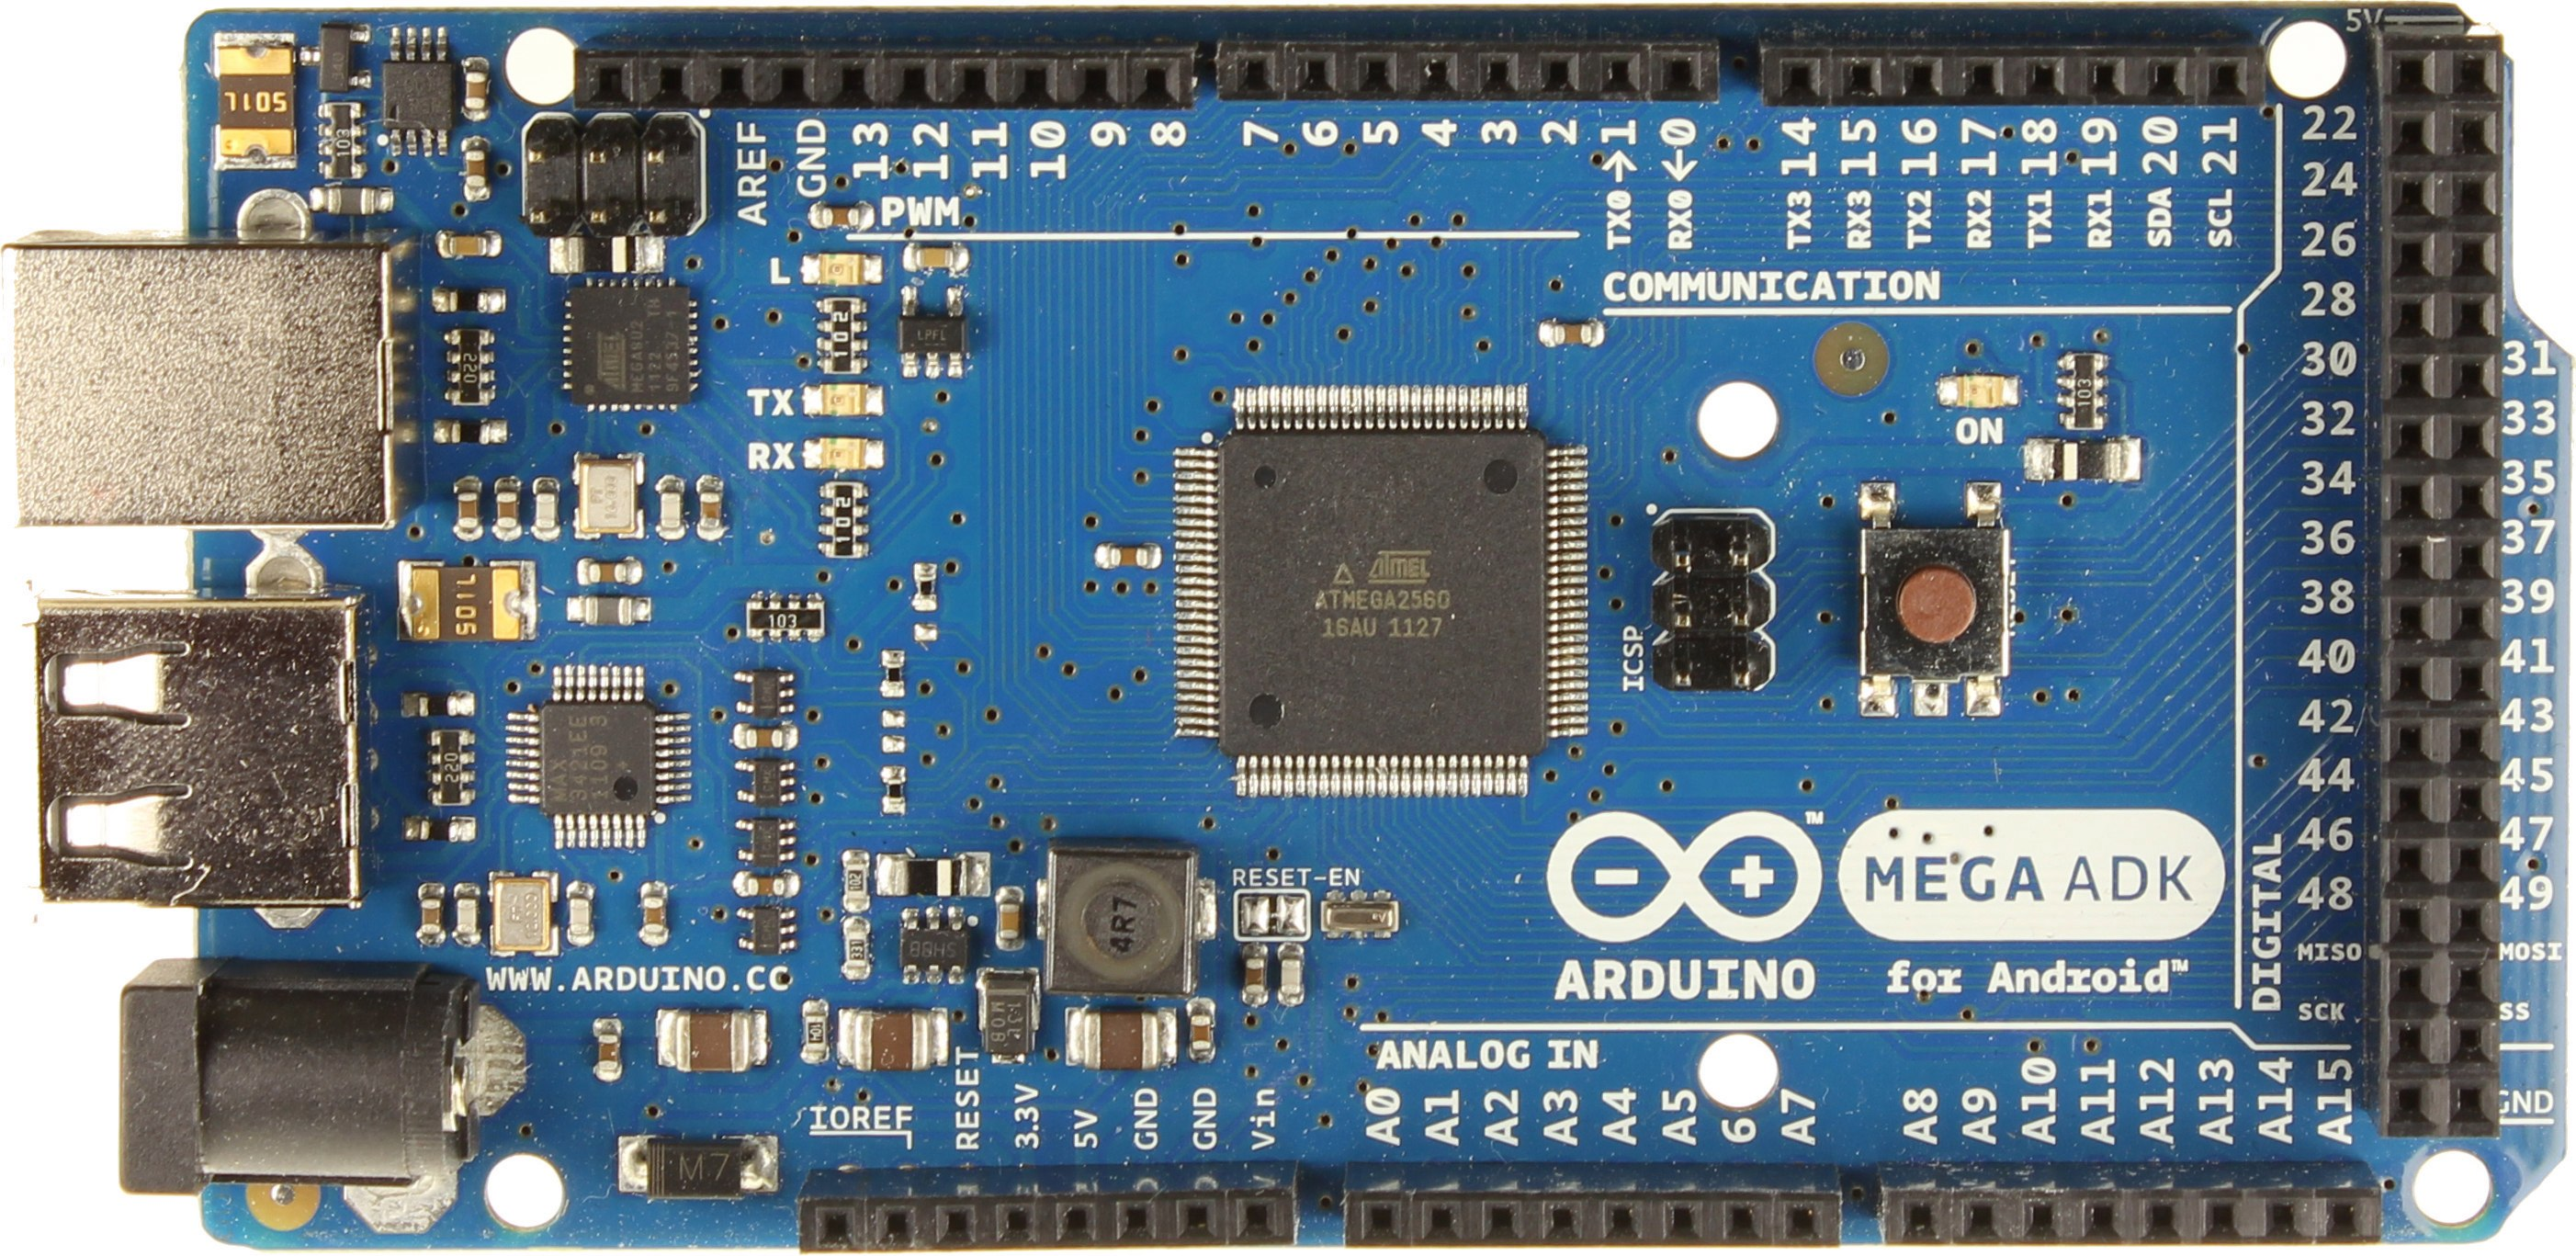
\includegraphics[height= 4cm, width=7cm]{project/images/ardunio}
  \caption{\textbf{Ardunio MEGA ADK}}
\end{figure}
\paragraph{}The Arduino Mega is a microcontroller board based on the ATmega1280 (datasheet). It has 54 digital input/output pins (of which 14 can be used as PWM outputs), 16 analog inputs, 4       UARTs (hardware serial ports), a 16 MHz crystal oscillator, a USB connection, a power jack, an ICSP header, and a reset button. It contains everything needed to support the microcontroller; simply connect it to a computer with a USB cable or power it with a AC-to-DC adapter or battery to get started. The Mega is compatible with most shields designed for the Arduino Duemilanove or Diecimila.
\large{\textbf{\\SUMMARY OF ARDUNIO}} 
\begin{enumerate}[a. ]
 \item Microcontroller ATmega1280
 \item Operating Voltage	5V
\item Input Voltage (recommended)	7-12V
\item Input Voltage (limits)	6-20V
\item Digital I/O Pins	54 (of which 15 provide PWM output)
\item Analog Input Pins	16
\item DC Current per I/O Pin	40 mA
\item DC Current for 3.3V Pin	50 mA
\item Flash Memory	128 KB of which 4 KB used by bootloader
\item SRAM	8 KB
\item EEPROM	4 KB
\item Clock Speed	16 MHz

\end{enumerate}

\section{Lazer}
\begin{figure}[H]
 \centering
    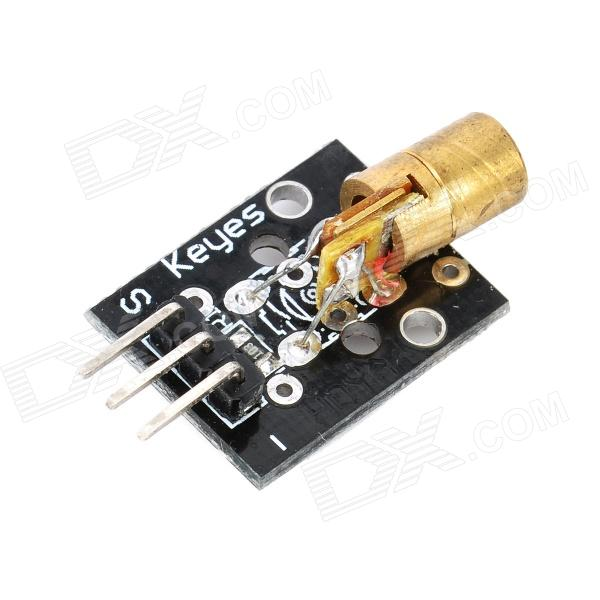
\includegraphics[height= 4cm, width=7cm]{project/images/lazer}
  \caption{\textbf{REES52 6 Psc Lazer}}
\end{figure}
\paragraph{}A laser is a device that emits light through a process of optical amplification based on the  stimulated  emission  of  electromagnetic  radiation.  The  term  "laser"  originated  as  an acronym for "light amplification by stimulated emission of radiation".
A laser differs from other sources of light in that it emits light coherently. Spatial coherence allows a laser to be focused to a tight spot, enabling applications such as laser cutting and lithography. Spatial coherence also allows a laser beam to stay narrow over great distances (collimation), enabling applications such as laser pointers. Lasers can also have high temporal coherence, which allows them to emit light with a very narrow spectrum, i.e., they can emit a single colour of light. Temporal coherence can be used to produce pulses of light as short as a femtosecond.


\section{GSM Module}

\begin{figure}[H]
 \centering
    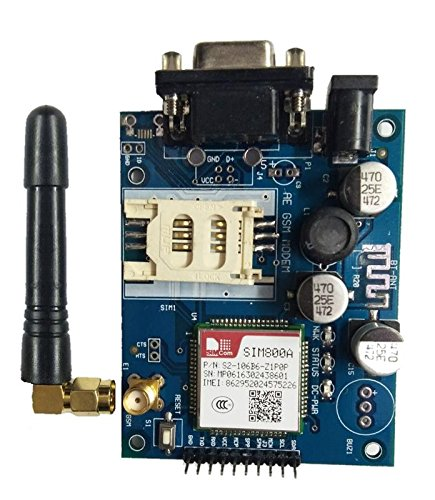
\includegraphics[height= 4cm, width=7cm]{project/images/sim module}
  \caption{\textbf{SIM 900}}
\end{figure}
\paragraph{}A GSM Module is basically a GSM Modem (like SIM 900) connected to a PCB with different types of output taken from the board – say TTL Output (for Arduino, 8051 and other microcontrollers) and RS232 Output to interface directly with a PC (personal computer). The board will also have pins or provisions to attach mic and speaker, to take out +5V or other values of power and ground connections. These type of provisions vary with different modules.Lots of varieties of GSM modem and GSM Modules are available in the market to choose from. For our project of connecting a gsm modem or module to arduino and hence send and receive sms using arduino – its always good to choose an arduino compatible GSM Module – that is a GSM module with TTL Output provisions.

\section{LDR}
\begin{figure}[H]
 \centering
    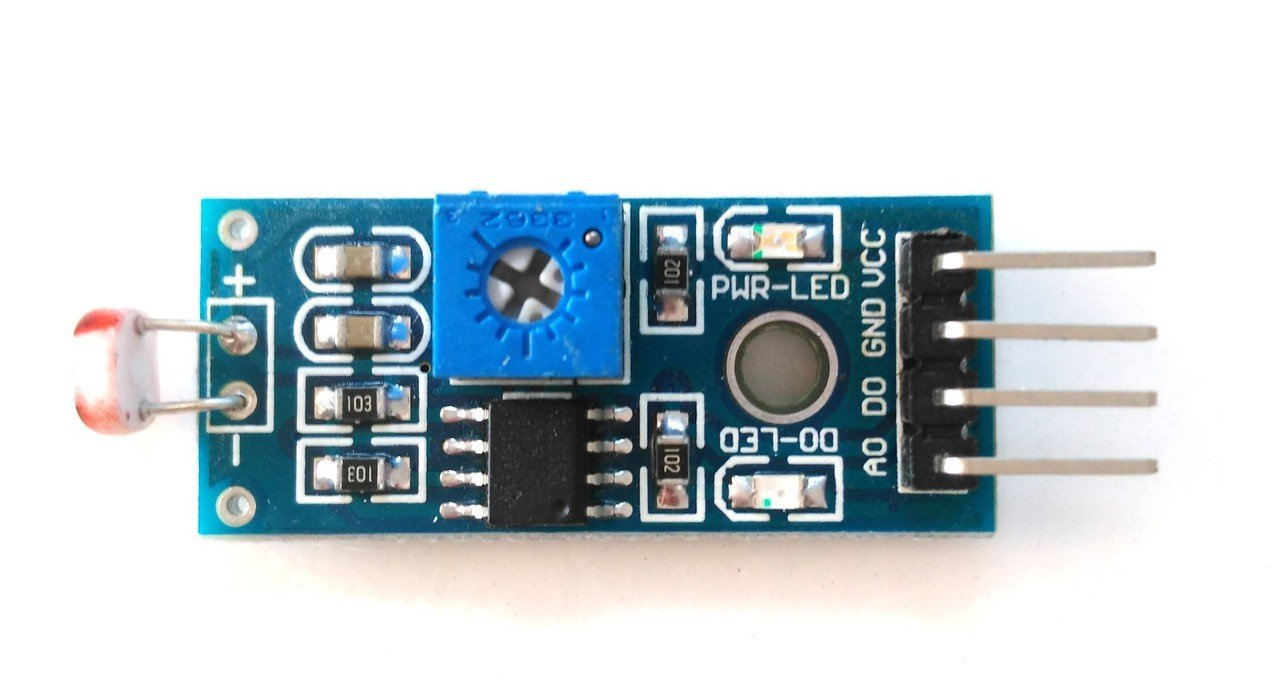
\includegraphics[height= 4cm, width=7cm]{project/images/LDR}
  \caption{\textbf{LDR}}
\end{figure}
\paragraph{}A Light Dependent Resistor (also known as a photoresistor or LDR) is a device whose resistivity is a function of the incident electromagnetic radiation. Hence, they are light-sensitive devices. They are also called as photoconductors, photoconductive cells or simply photocells.They are made up of semiconductor materials that have high resistance. There are many different symbols used to indicate a photoresistor or LDR, one of the most commonly used symbol is shown in the figure below. The arrow indicates light falling on it.Those semiconductor materials which have a direct band gap are the ones that emit photons. When a suitable voltage is applied to the leads, electrons are able to recombine with electron holes within the device, releasing energy in the form  of  photons.  This  effect  is called  electroluminescence  and  the  colour  of  the  light (corresponding to the energy of the photon) is determined by the energy band gap of the semiconductor. An LED is often small in area (less  than I mm2) and integrated optical components may be used to shape its radiation pattern

\section{Buzzer}
\begin{figure}[H]
 \centering
    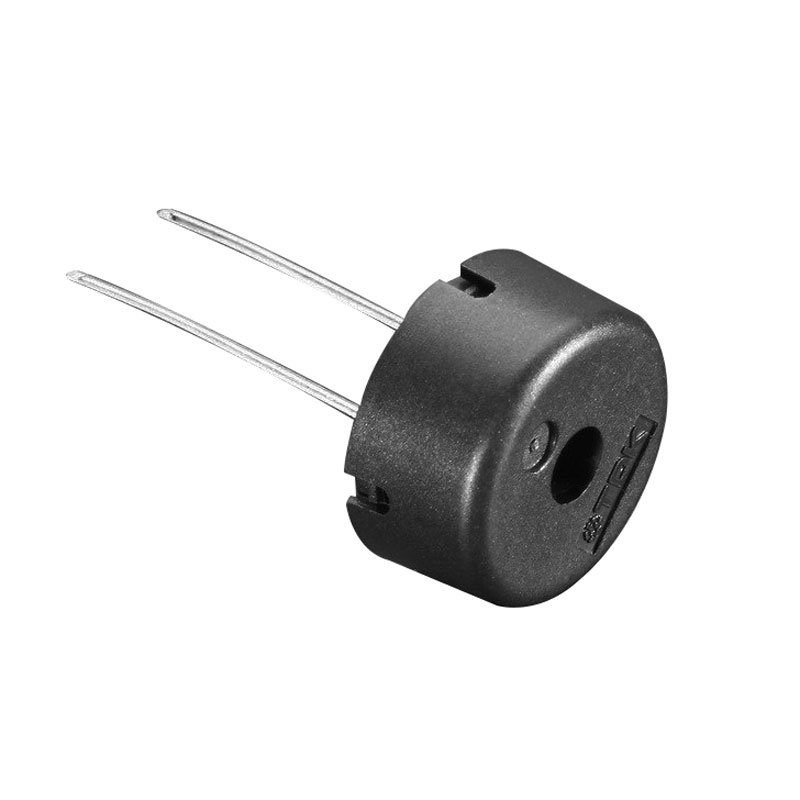
\includegraphics[height= 4cm, width=7cm]{project/images/buzzer}
  \caption{\textbf{buzzer}}
\end{figure}
\paragraph{}A  buzzer  or  beeper  is  an  audio  signalling  device,  which  may  be  mechanical, electromechanical, and piezoelectric. Typical uses of buzzers and beepers  include  alarm devices, timers and confirmation of user input such as a mouse click or keystroke.
Early devices were based on an electromechanical system identical to an electric bell without the metal gong. Similarly, a relay may be connected to interrupt its own actuating current, causing the contacts to buzz. Often these units were anchored to a wall or ceiling to use it as a sounding board. The word "buzzer" comes from the rasping noise that electromechanical buzzers made.
The buzzer consists of an outside case with two pins to attach it to power and ground.  When current is applied to the buzzer it causes the ceramic disk to contract or expand. Changing this then causes the surrounding disc to vibrate. That's the sound that you hear. Adjust the potentiometer to increase or decrease the resistance of the potentiometer. If you increase the resistance of the potentiometer then it will decrease the Volume of the buzzer. If you decrease the resistance of the potentiometer then it will increase the Volume of the buzzer.



\chapter{Arduino Cicuit Design}
\section{Establish Connection}
\begin{figure}[H]
 \centering
    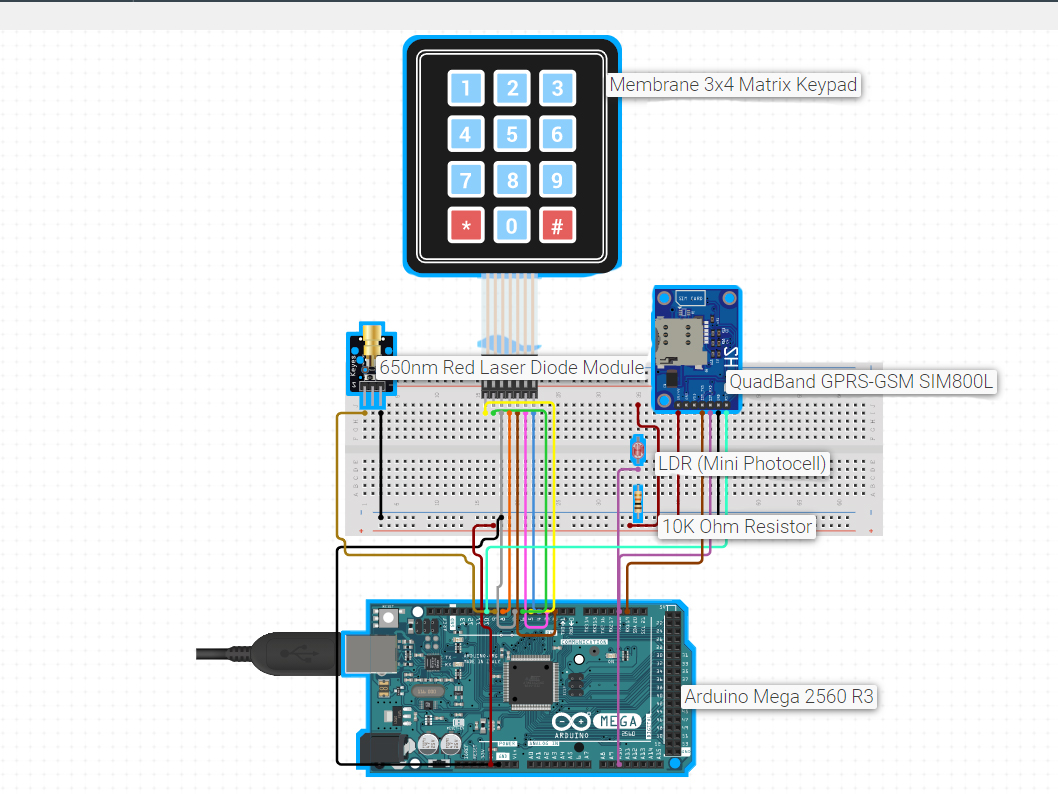
\includegraphics[height= 10cm, width=13cm]{project/images/circuit diagram}
  \caption{\textbf{Arduino Cicuit Design}}
\end{figure}
\paragraph{}1. We use SIM900 GSM Module – This means the module supports communication in 900MHz band. We are from India and most of the mobile network providers in this country operate in the 900Mhz band. If you are from another country, you have to check the mobile network band in your are
\paragraph{}2.Check the power requirements of GSM module – GSM modules are manufactured by different companies. They all have different input power supply specs. You need to double check your GSM modules power requirements.
\paragraph{}3.Our gsm module requires a 12 volts input. So we feed it using a 12V,1A DC power supply. I have seen gsm modules which require 15 volts and some other types which needs only 5 volts input. They differ with manufacturers. If you are having a 5V module, you can power it directly from Arduino’s 5V out.
\paragraph{}4.Check for TTL Output Pins in the module – You can feed the data from gsm module directly to Arduino only if the module is enabled with TTL output pins. Otherwise you have to convert the RS232 data to TTL using MAX232 IC and feed it to Arduino. Most of the gsm modules in market are equipped with TTL output pins. Just ensure you are buying the right one.
\paragraph{}
\textbf{Booting the GSM Module}
\paragraph{}1. Insert the SIM card to GSM module and lock it.

\paragraph{}2.Connect the adapter to GSM module and turn it ON!

\paragraph{}3.Now wait for some time (say 1 minute) and see the blinking rate of ‘status LED’  or ‘network LED’ (GSM module will take some time to establish connection with mobile network)

\paragraph{}4.Once the connection is established successfully, the status/network LED will blink continuously every 3 seconds.
\begin{figure}[H]
 \centering
    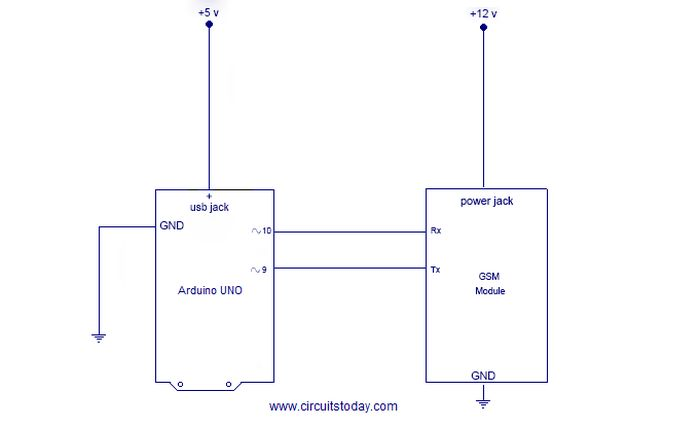
\includegraphics[height= 7cm, width=9cm]{project/images/cir}
  \caption{\textbf{Arduino and GSM Module Block Daigram}}
\end{figure}
\paragraph{}

\textbf{\\Other Connection}
\paragraph{} 1)GSM Module TXD pin in Connect to the Digital pin no 2 
\paragraph{} 2)GSM Module RXD pin in Connect to the Digital pin no 3 
\paragraph{}
\textbf{A)Buzzer Connection}
\paragraph{}1)Connnect Positive pin of Buzzer to the Digital pin no 12
\paragraph{}2)Connnect Negative pin of Buzzer to the Digital pin 3.3v
\paragraph{}
\textbf{B)Lazer Connection}
\paragraph{}1)Connnect Pin Ground to Ground
\paragraph{}2)Connnect VCC in 5v
\paragraph{}
\textbf{C)Keypad Connection}
\paragraph{}
\begin{table}[H]
\centering
\begin{tabular}{|c|c|}
\hline
4 X 4 Keypad & Arduino           \\ \hline
R1           & \textbf{$\sim$11} \\ \hline
R2           & \textbf{$\sim$10} \\ \hline
\textbf{R3}  & \textbf{$\sim$9}  \\ \hline
\textbf{R4}  & \textbf{8}        \\ \hline
\textbf{C1}  & \textbf{7}        \\ \hline
\textbf{C2}  & \textbf{$\sim$6}  \\ \hline
\textbf{C3}  & \textbf{$\sim$5}  \\ \hline
\textbf{C4}  & \textbf{4}        \\ \hline
\end{tabular}
\caption{Connection of Keypad and Arduino}
\end{table}



\input{project/testing.tex}

\chapter{ADVANTAGES AND DISADVANTAGES}
\section{ADVANTAGES:}
\paragraph{}
These are easy to install and work at both within as well as outside houses. These are very effective perimeter alarm systems around properties. In indoor systems can utilize the normal power outlets and jacks making them inconspicuous. At outside these can be easily be hidden behind the bushes or plants without causing any damage. They consume less power when compared to the laser system as the whole, which is expensive.
These laser systems can be installed in homes either by self or by hiring a technical person. By technological innovations cost of the security systems has been cut to a large extent. So, making laser systems one among affordable security system options can be very safe.
Lasers are strong in beam width and can be focused on the perfect target. By using laser security system one can be safe in the case of harmful effects to the body. As the beam width used in the laser security systems are not strong beam widths. 
The circuit, construction and setup for the Laser Security System are very simple. If used with a battery, the laser security system can work even when there is a power outage.
\paragraph{}
\section{DISADVANTAGES:}

a)The laser security system works only if the laser is obstructed. If the intruder passes without obstructing the laser, it is considered as a failure.
\\
b)In order to secure a larger area, we need more lasers and corresponding sensors.
\chapter{Program}
\paragraph{}The open-source Arduino Software (IDE) makes it easy to write code and upload it to the board. It runs on Windows, Mac OS X, and Linux. The environment is written in Java and based on Processing and other open-source software. This software can be used with any Arduino board.

\begin{figure}[H]
 \centering
    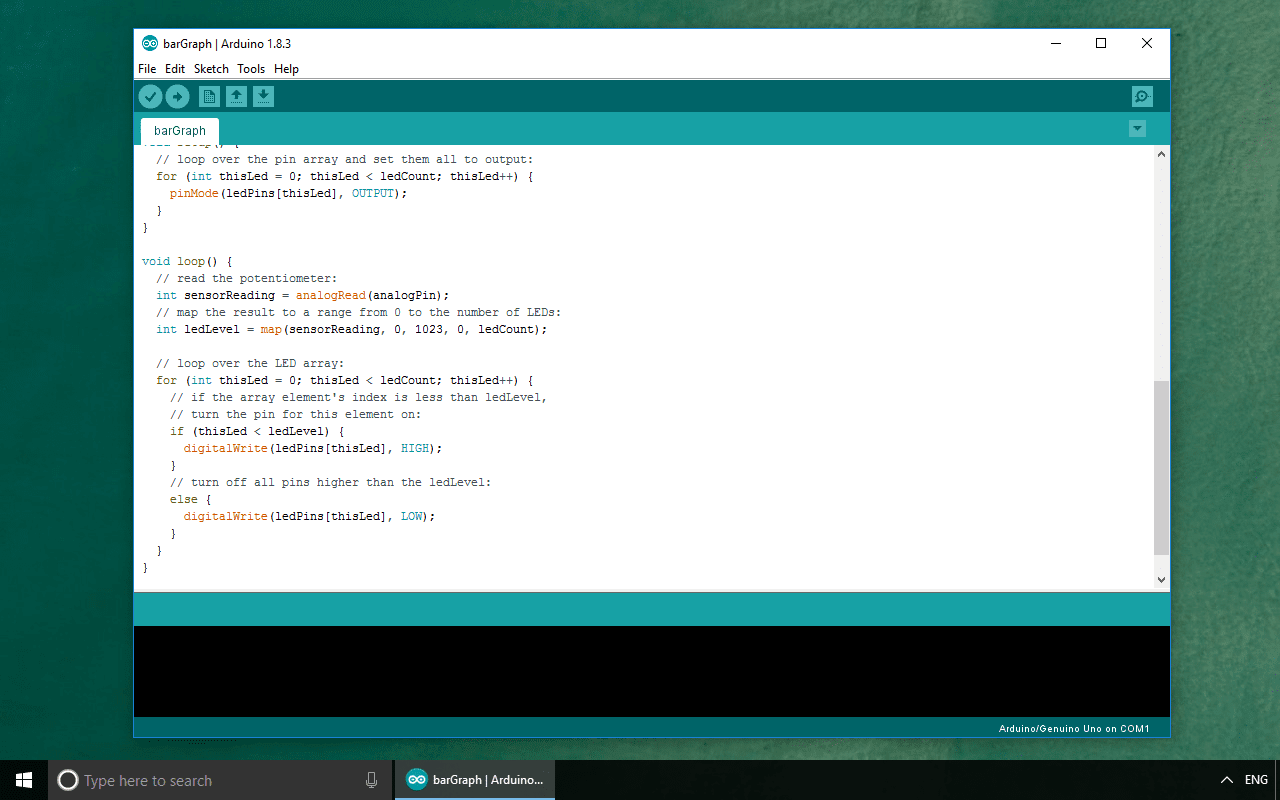
\includegraphics[height= 7cm, width=13cm]{project/images/ide}
  \caption{\textbf{Arduino Coding IDE}}
\end{figure}

\begin{lstlisting}
  #include <Keypad.h>
#include <LiquidCrystal.h>
#include<SoftwareSerial.h>;
SoftwareSerial gsm(2,3);
const int ldr_pin = A0;

const byte ROWS = 4; //four rows
const byte COLS = 4; //three columns
char keys[ROWS][COLS] = {
  {'1','2','3'},
  {'4','5','6'},
  {'7','8','9'},
  {'*','0','#'}
};
byte rowPins[ROWS] = {4,5,6,7}; //connect to the row pinouts of the keypad
byte colPins[COLS] = {8,9,10,11}; //connect to the column pinouts of the keypad
 
Keypad keypad = Keypad( makeKeymap(keys), rowPins, colPins, ROWS, COLS );
 

String password = "1234";
String mypassword;
 
int lock = 13;
 
int counter = 0; 
int attempts = 0; 
int max_attempts = 3; 
 
void setup(){
  Serial.begin(9600);
  // set up the LCD's number of columns and rows: 
 
  
 
  pinMode(lock, OUTPUT);
  pinMode(12,OUTPUT);
   pinMode(ldr_pin,INPUT);
  digitalWrite(12,HIGH);
 
  digitalWrite(lock, LOW);
  
  Serial.println("enter password");
    
}
  
void loop()
{
  
 keypadfunction();
 ldr();
 
}
 
void keypadfunction()
{
 char key = keypad.getKey();
  
  if (key){
    Serial.println(key);
    
  }
  if (key == '1')
  {
 
    mypassword = mypassword + 1;   
  }
  
    if (key == '2')
  {
 
    mypassword = mypassword + 2;  
  }
  
  if (key == '3')
  {
 
    mypassword = mypassword + 3; 
  }
  
   if (key == '4')
  {
  
    mypassword = mypassword + 4;  
  }
  
  if (key == '5')
  {
  
    mypassword = mypassword + 5;
  }
  
   if (key == '6')
  {
   
    mypassword = mypassword + 6; 
  }
  
   if (key == '7')
  {
 
    mypassword = mypassword + 7; 
  }
 
   if (key == '8')
  {
 
    mypassword = mypassword + 8; 
  }
  
  if (key == '9')
  {
 
    mypassword = mypassword + 9;
  }
             
                 if (key == '0')
  {
 
    mypassword = mypassword + 0; 
  }
  
  
        if (key == '*')
  {
    Serial.println(mypassword); 
    
if ( password == mypassword )
{
Serial.print(""); 
Serial.println("SYSTEM UNLOCKED");

Serial.println("WELCOME OWNER");
digitalWrite(lock, HIGH);
delay(50000                                                                                                                                               ); 
digitalWrite(lock,LOW);
mypassword = ""; 
counter = 0;  
Serial.println("Enter password");
}
else
{
Serial.println("wrong");

attempts = attempts + 1; 
if (attempts >= max_attempts )
{
  Serial.print("");
  call();
  digitalWrite(12,HIGH);
   
  Serial.print("Locked Out");
  

delay(5000); 
 
attempts = 0; 

}
mypassword = ""; 
counter = 0; 
Serial.print(""); 
 
Serial.print("Wrong Password");
delay(1000);

 
Serial.print("max attempts 3");
delay(1000);

Serial.print(""); 
Serial.println("Enter password");
 
}
    
  }  
  
  
}
void ldr()
{
  int ldrStatus = analogRead(ldr_pin);
  

if (ldrStatus <= 200) {

digitalWrite(12, LOW);


} else {
digitalWrite(12, HIGH);
call();
delay(5000);




}


  }
void call()
{
  gsm.begin(9600);
  gsm.println("ATD+918380843911;"); //replace x by your number
  delay(100);
  gsm.println("ATH");

  }
\end{lstlisting}
\newpage

 % adds the Project Design
\chapter{Screenshots of Project}
\section{WHEN PASSWORD ENTERING}
\vspace{2cm}
\begin{figure}[H]
  \centering
    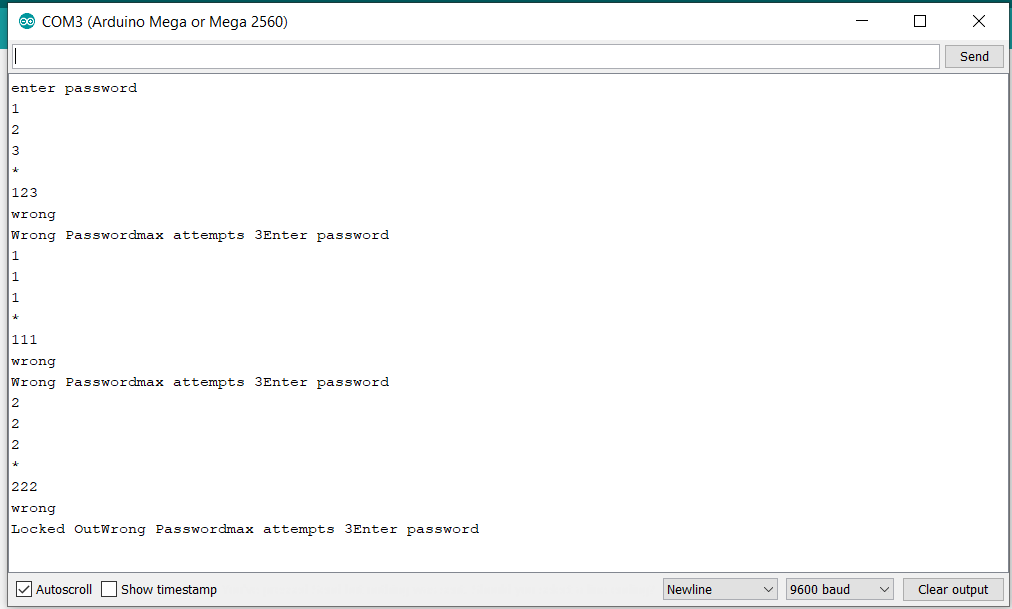
\includegraphics[height= 8cm, width=12cm]{project/images/WrongPassword}
    \caption{\textbf { When Entering Wrong Password}}
\end{figure}
\paragraph{}\textbf{ \color{red} NOTE:- Suppose if a person enters the wrong password 3 TIMES, a call will come in a few moments and an alarm will sound}
\newpage
\begin{figure}[H]
  \centering
    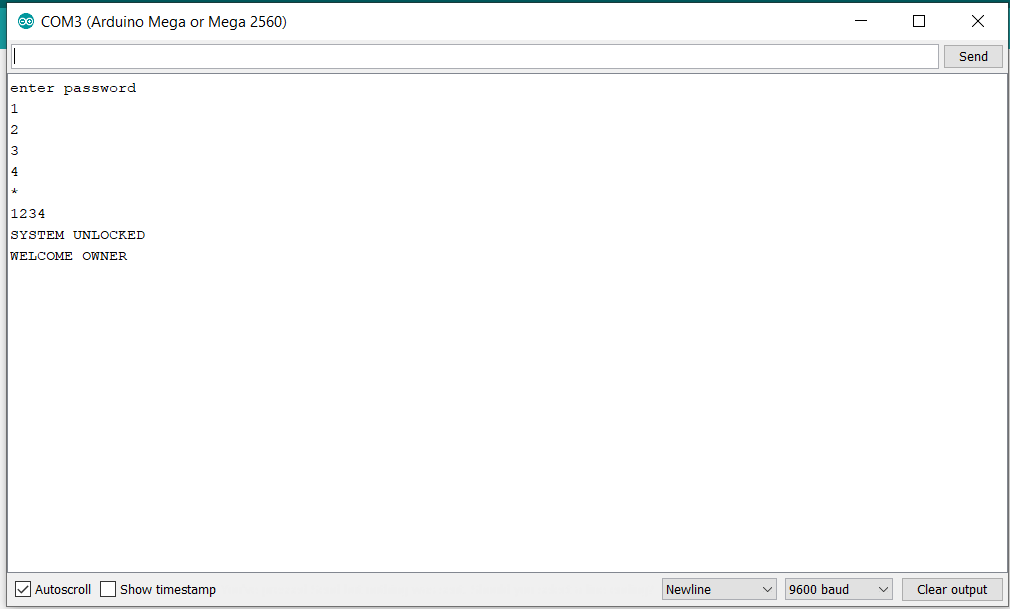
\includegraphics[height= 8cm, width=12cm]{project/images/currectPassword}
     \caption{\textbf { When Entering Correct Password}}
     
\end{figure}
\paragraph{}\textbf{\color{red} NOTE:-The internal laser system will automatically shut down for 1 minute when you enter the password correctly}
\vspace{1cm}

\begin{figure}[H]
  \centering
    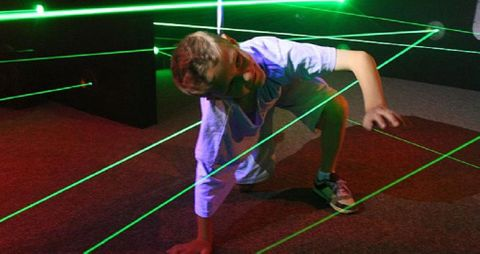
\includegraphics[height= 8cm, width=10cm]{project/images/cross}
    \caption{\textbf {When someone try CROSS the lazer security system}}
\end{figure}
\paragraph{}\textbf{\color{red}NOTE:-When someone enters and cross the LAZER, a call and Buzzer alert  will appear on the mobile in a few moments}


\begin{figure}[H]
  \centering
    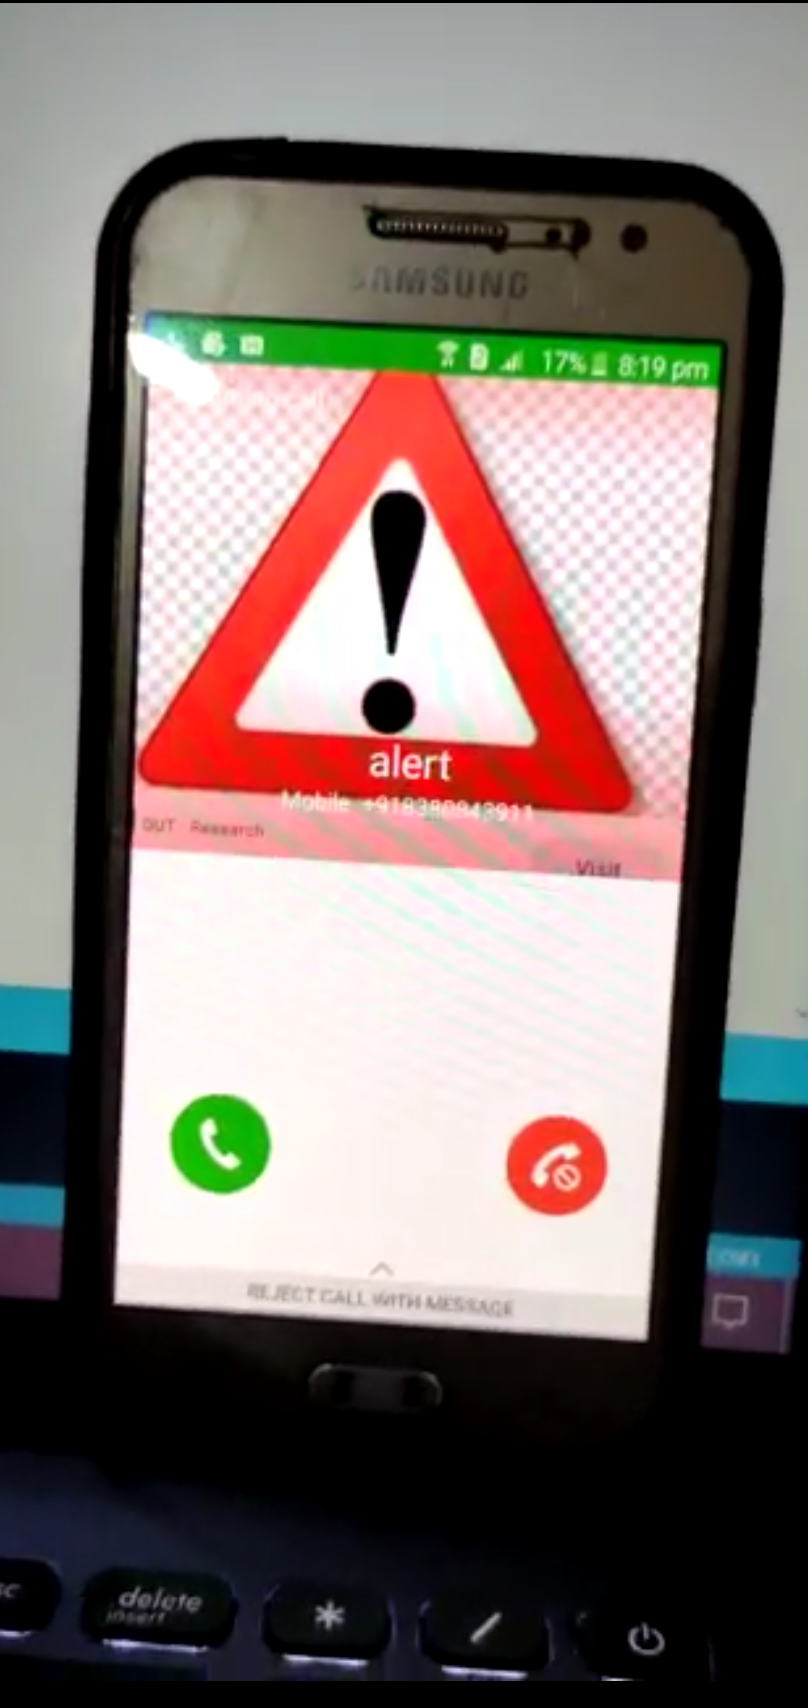
\includegraphics[height= 8cm, width=10cm]{project/images/Screenshot (321)}
    \caption{\textbf {Show The Alert Through Mobile}}
\end{figure}
\paragraph{}\textbf{\color{red}NOTE:-When someone enters the wrong password 3 TIMES and crosse the LAZER, a call alert will appear on the mobile in a few moments}
\section{Model Image}
\begin{figure}[H]
  \centering
    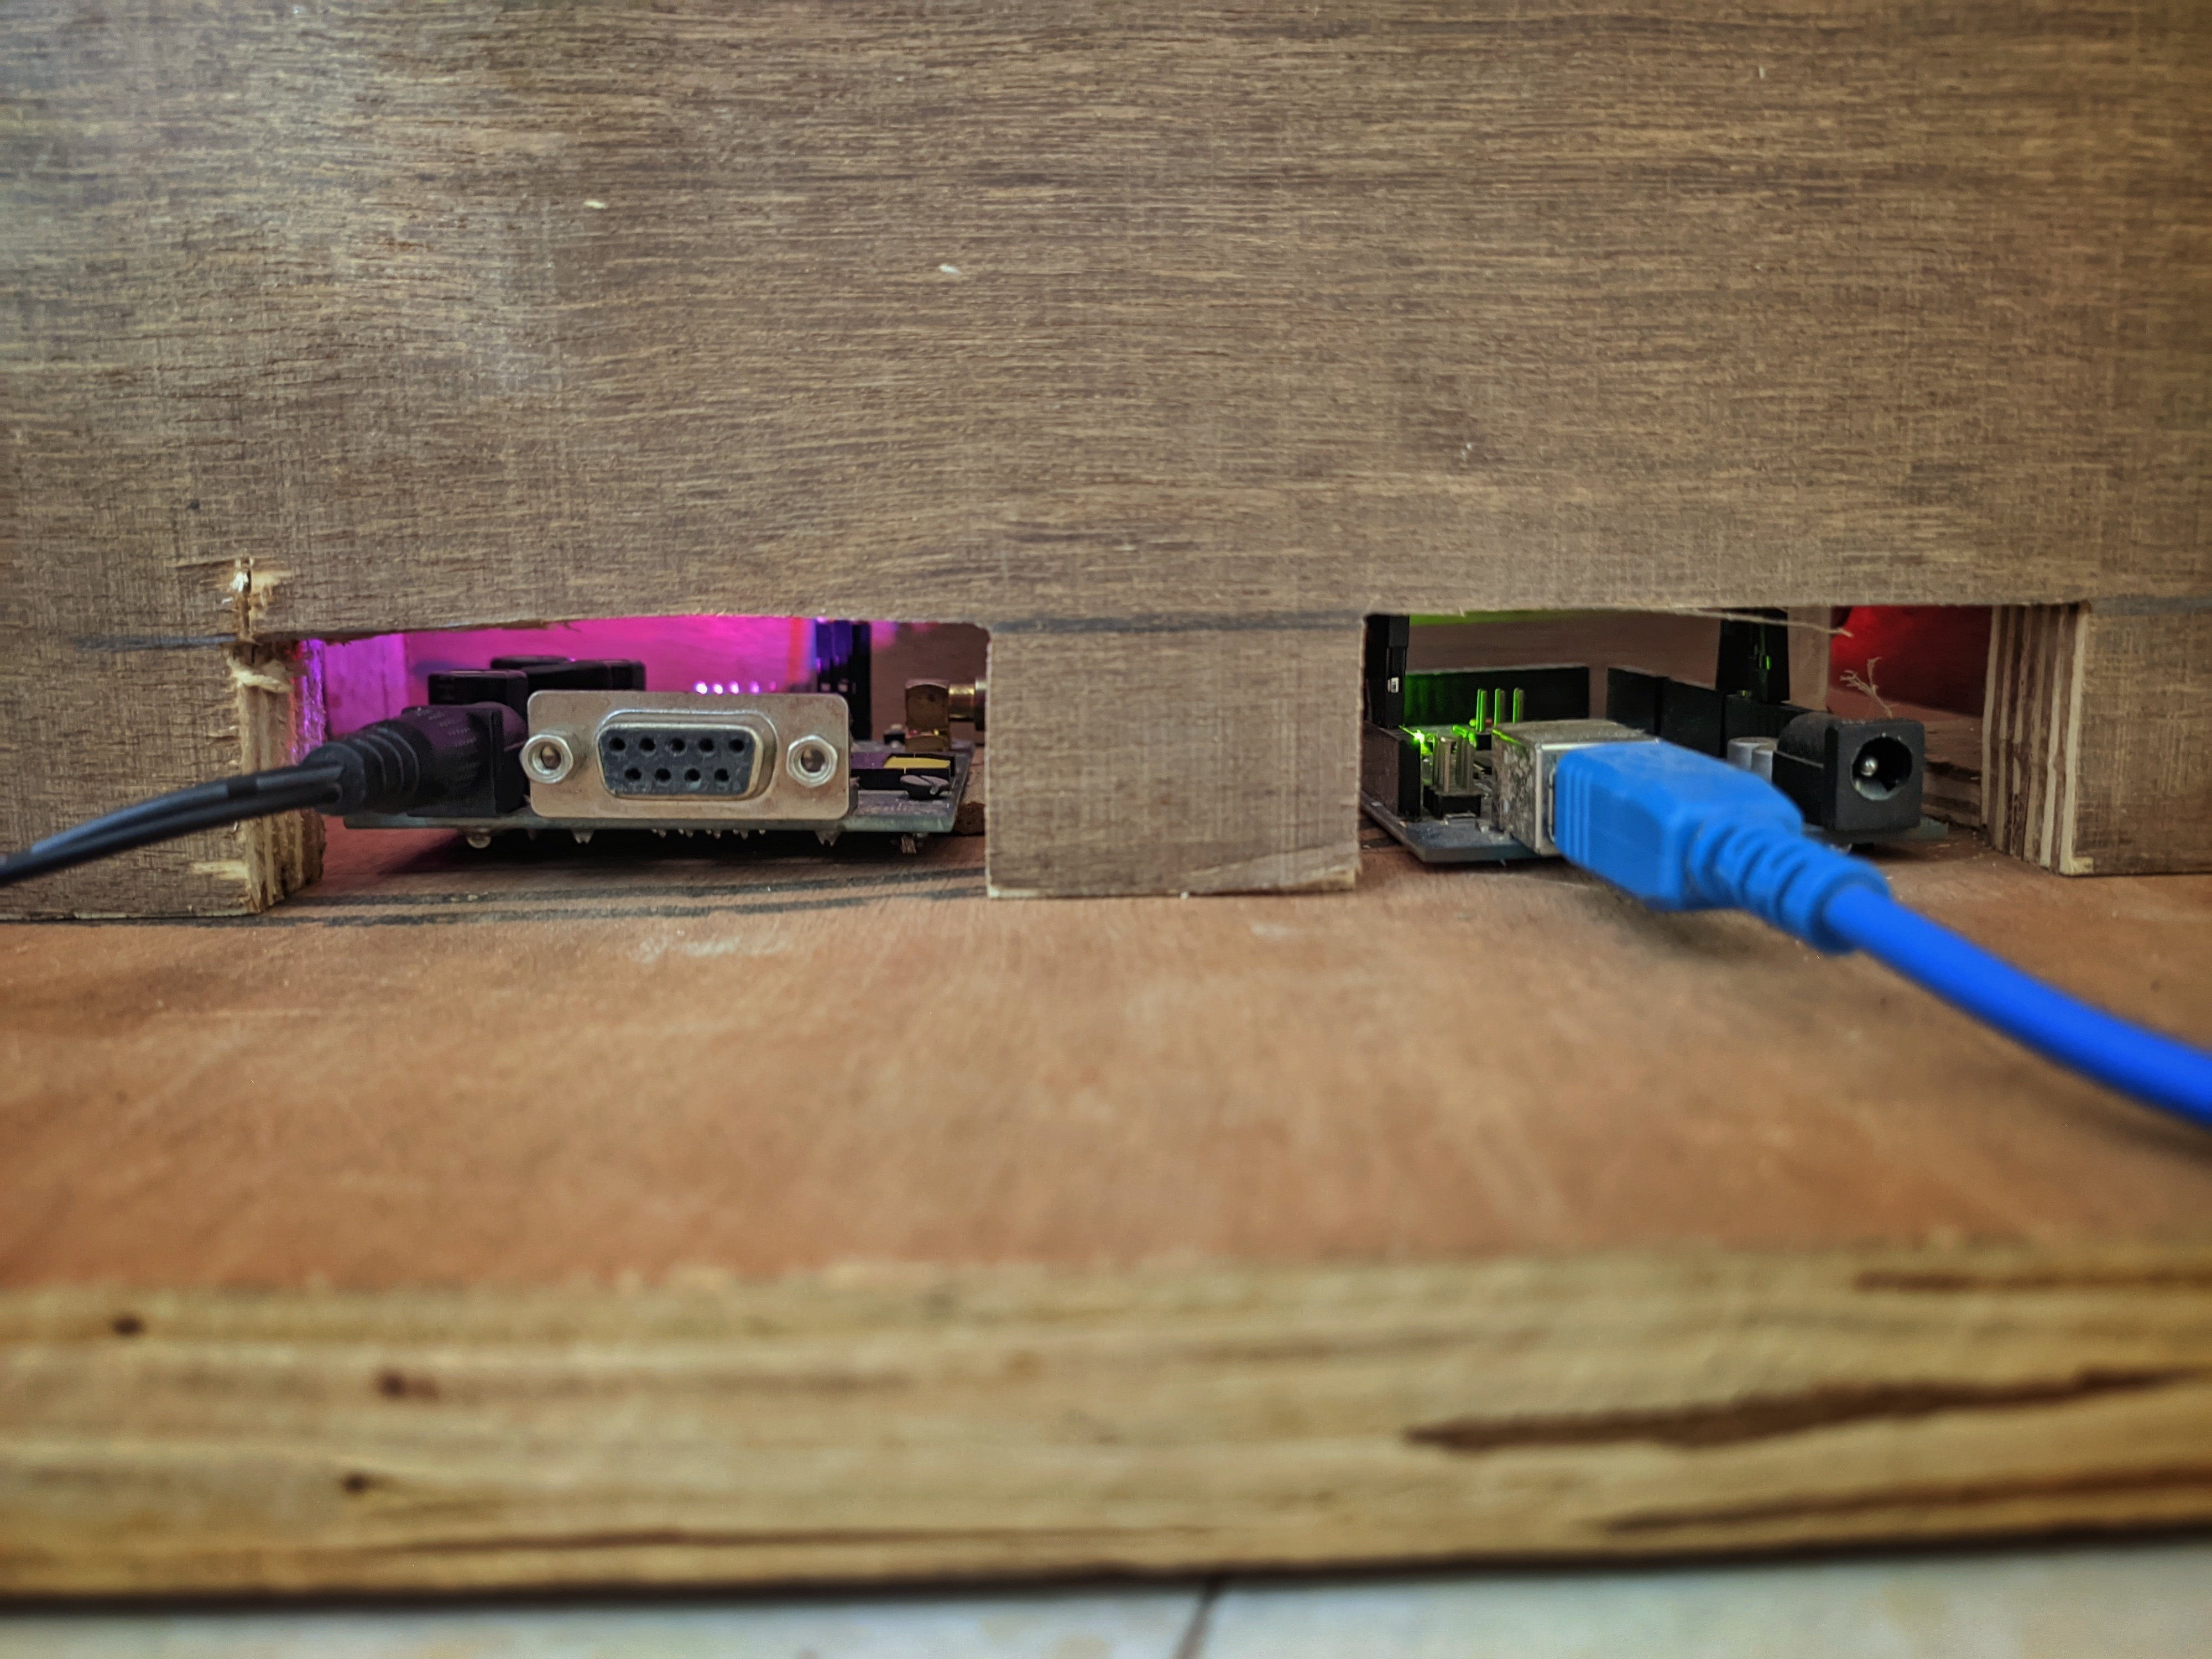
\includegraphics[height= 6cm, width=10cm]{project/images/img1}
    \caption{\textbf {connetion of GSM and arduino }}
\end{figure}
\begin{figure}[H]
  \centering
    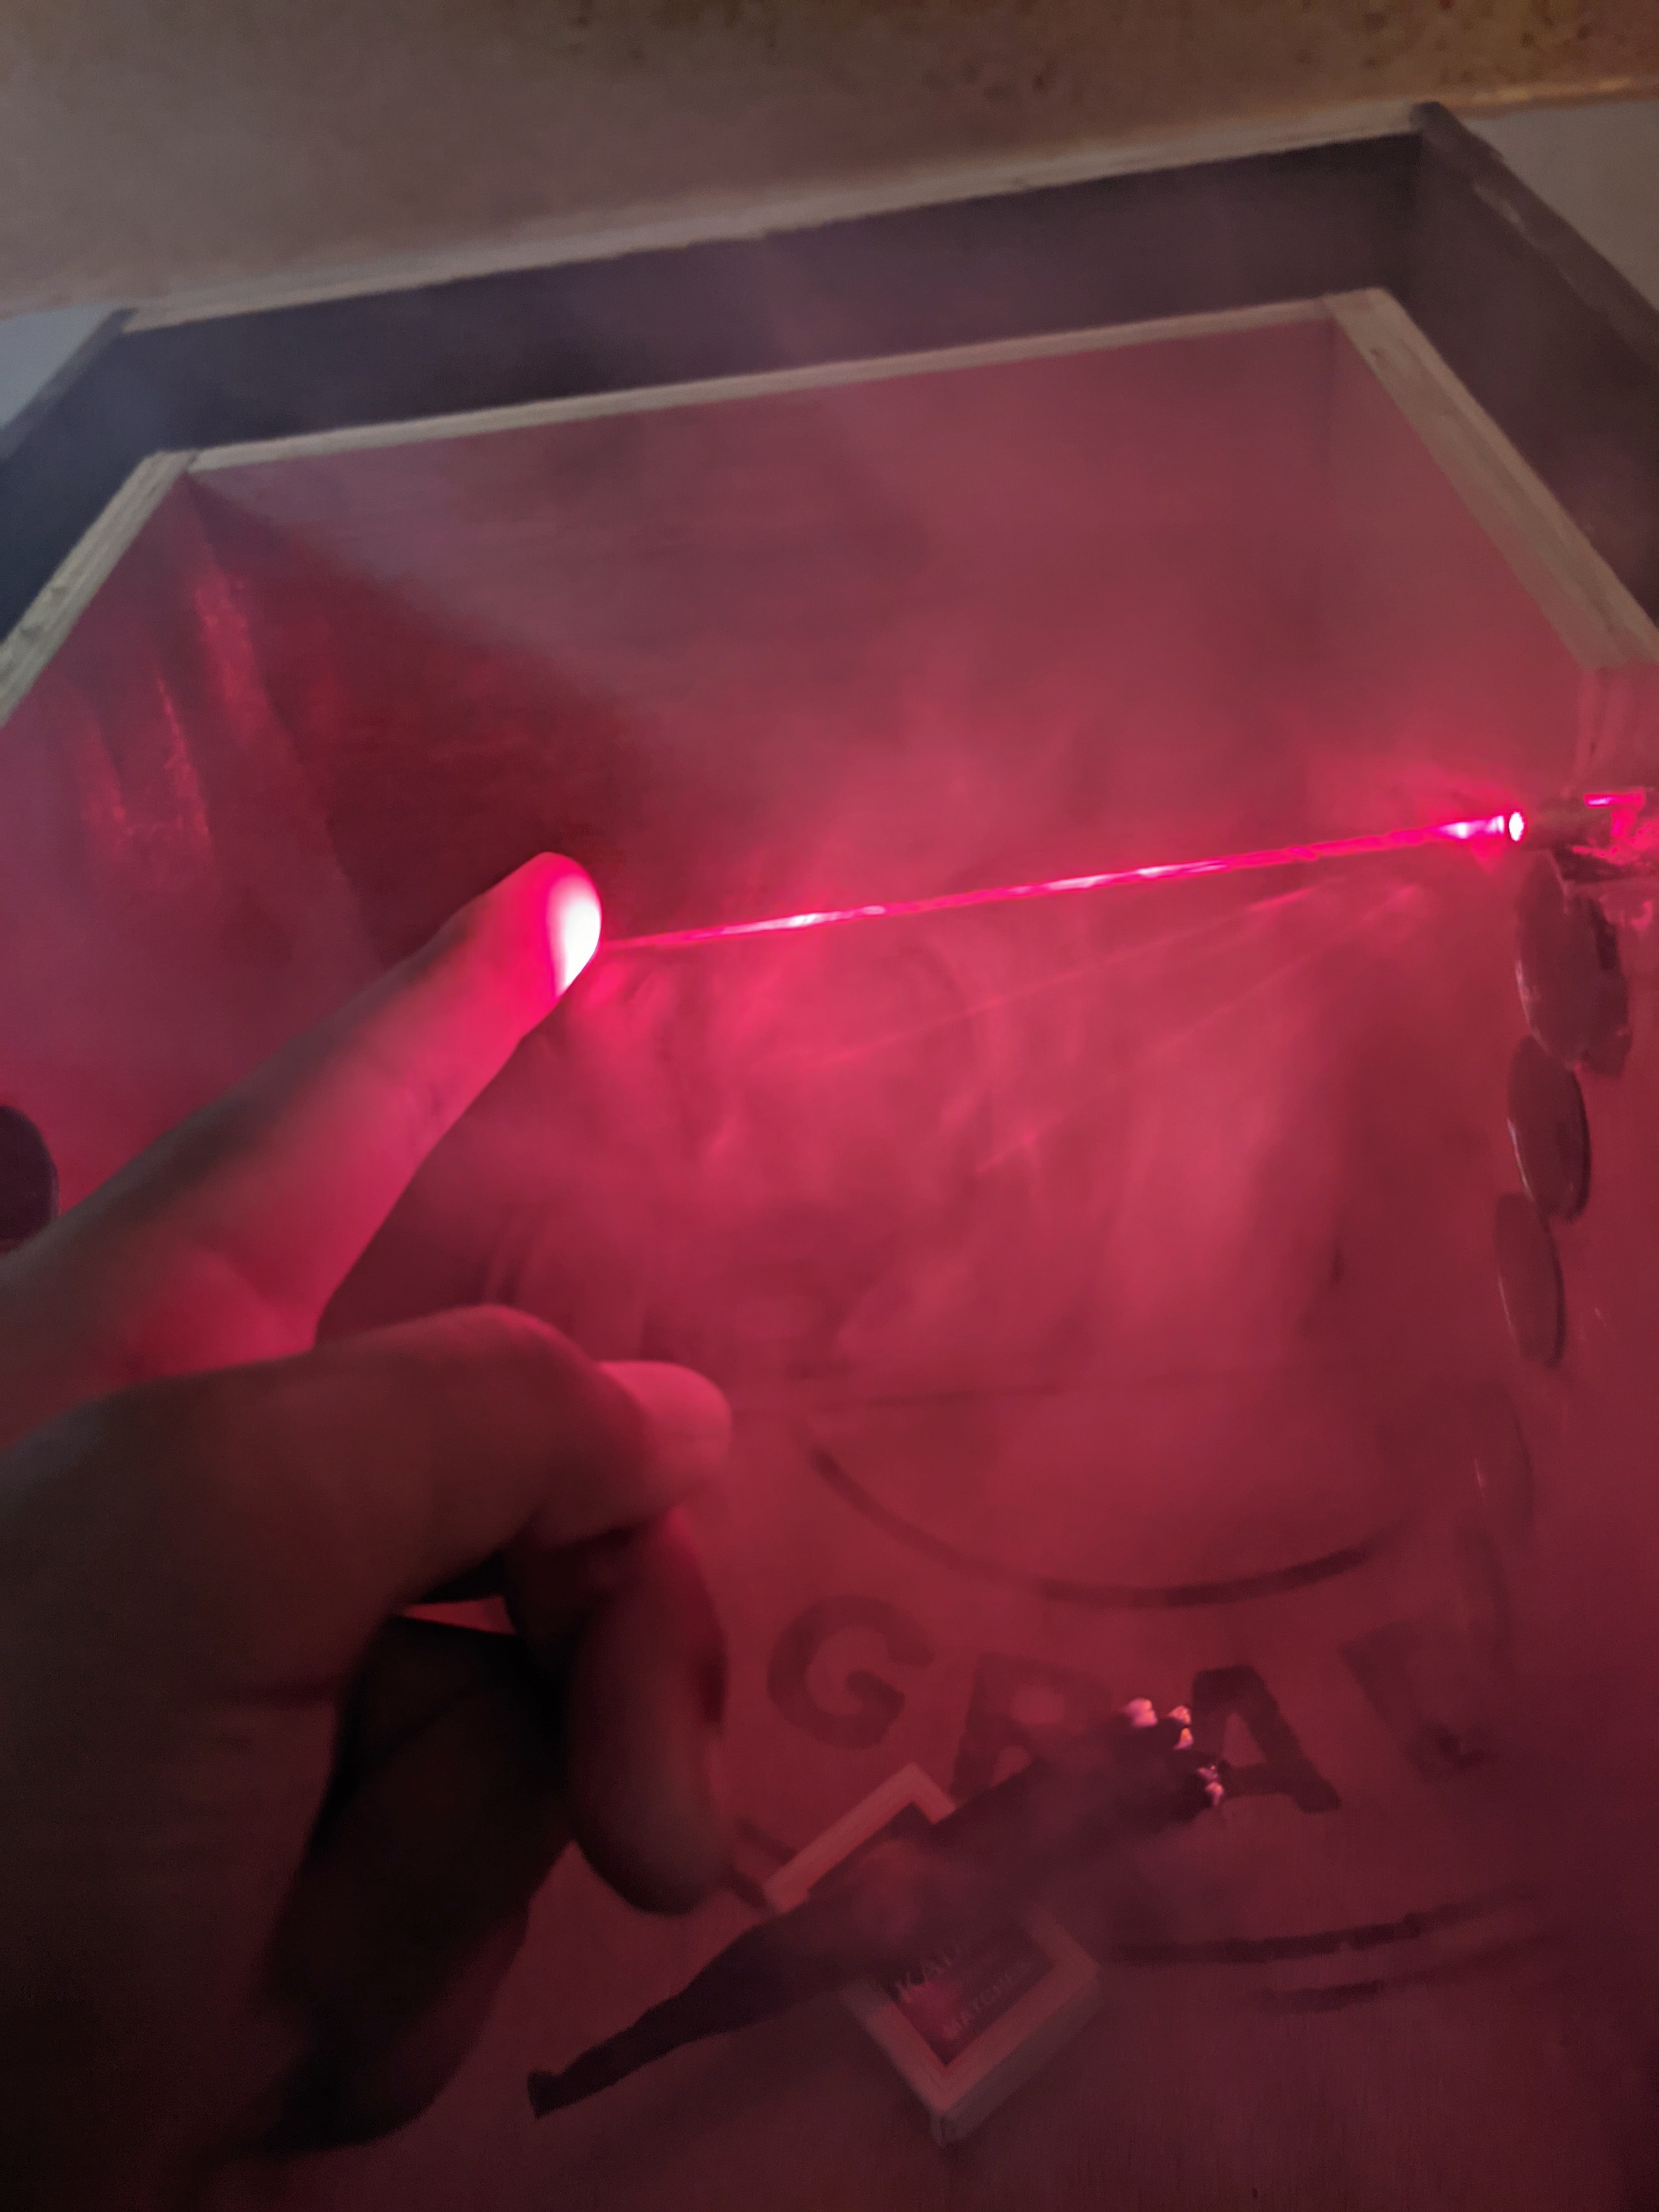
\includegraphics[height= 6cm, width=10cm]{project/images/img2}
    \caption{\textbf {lazer working in smoke }}
\end{figure}
\begin{figure}[H]
  \centering
    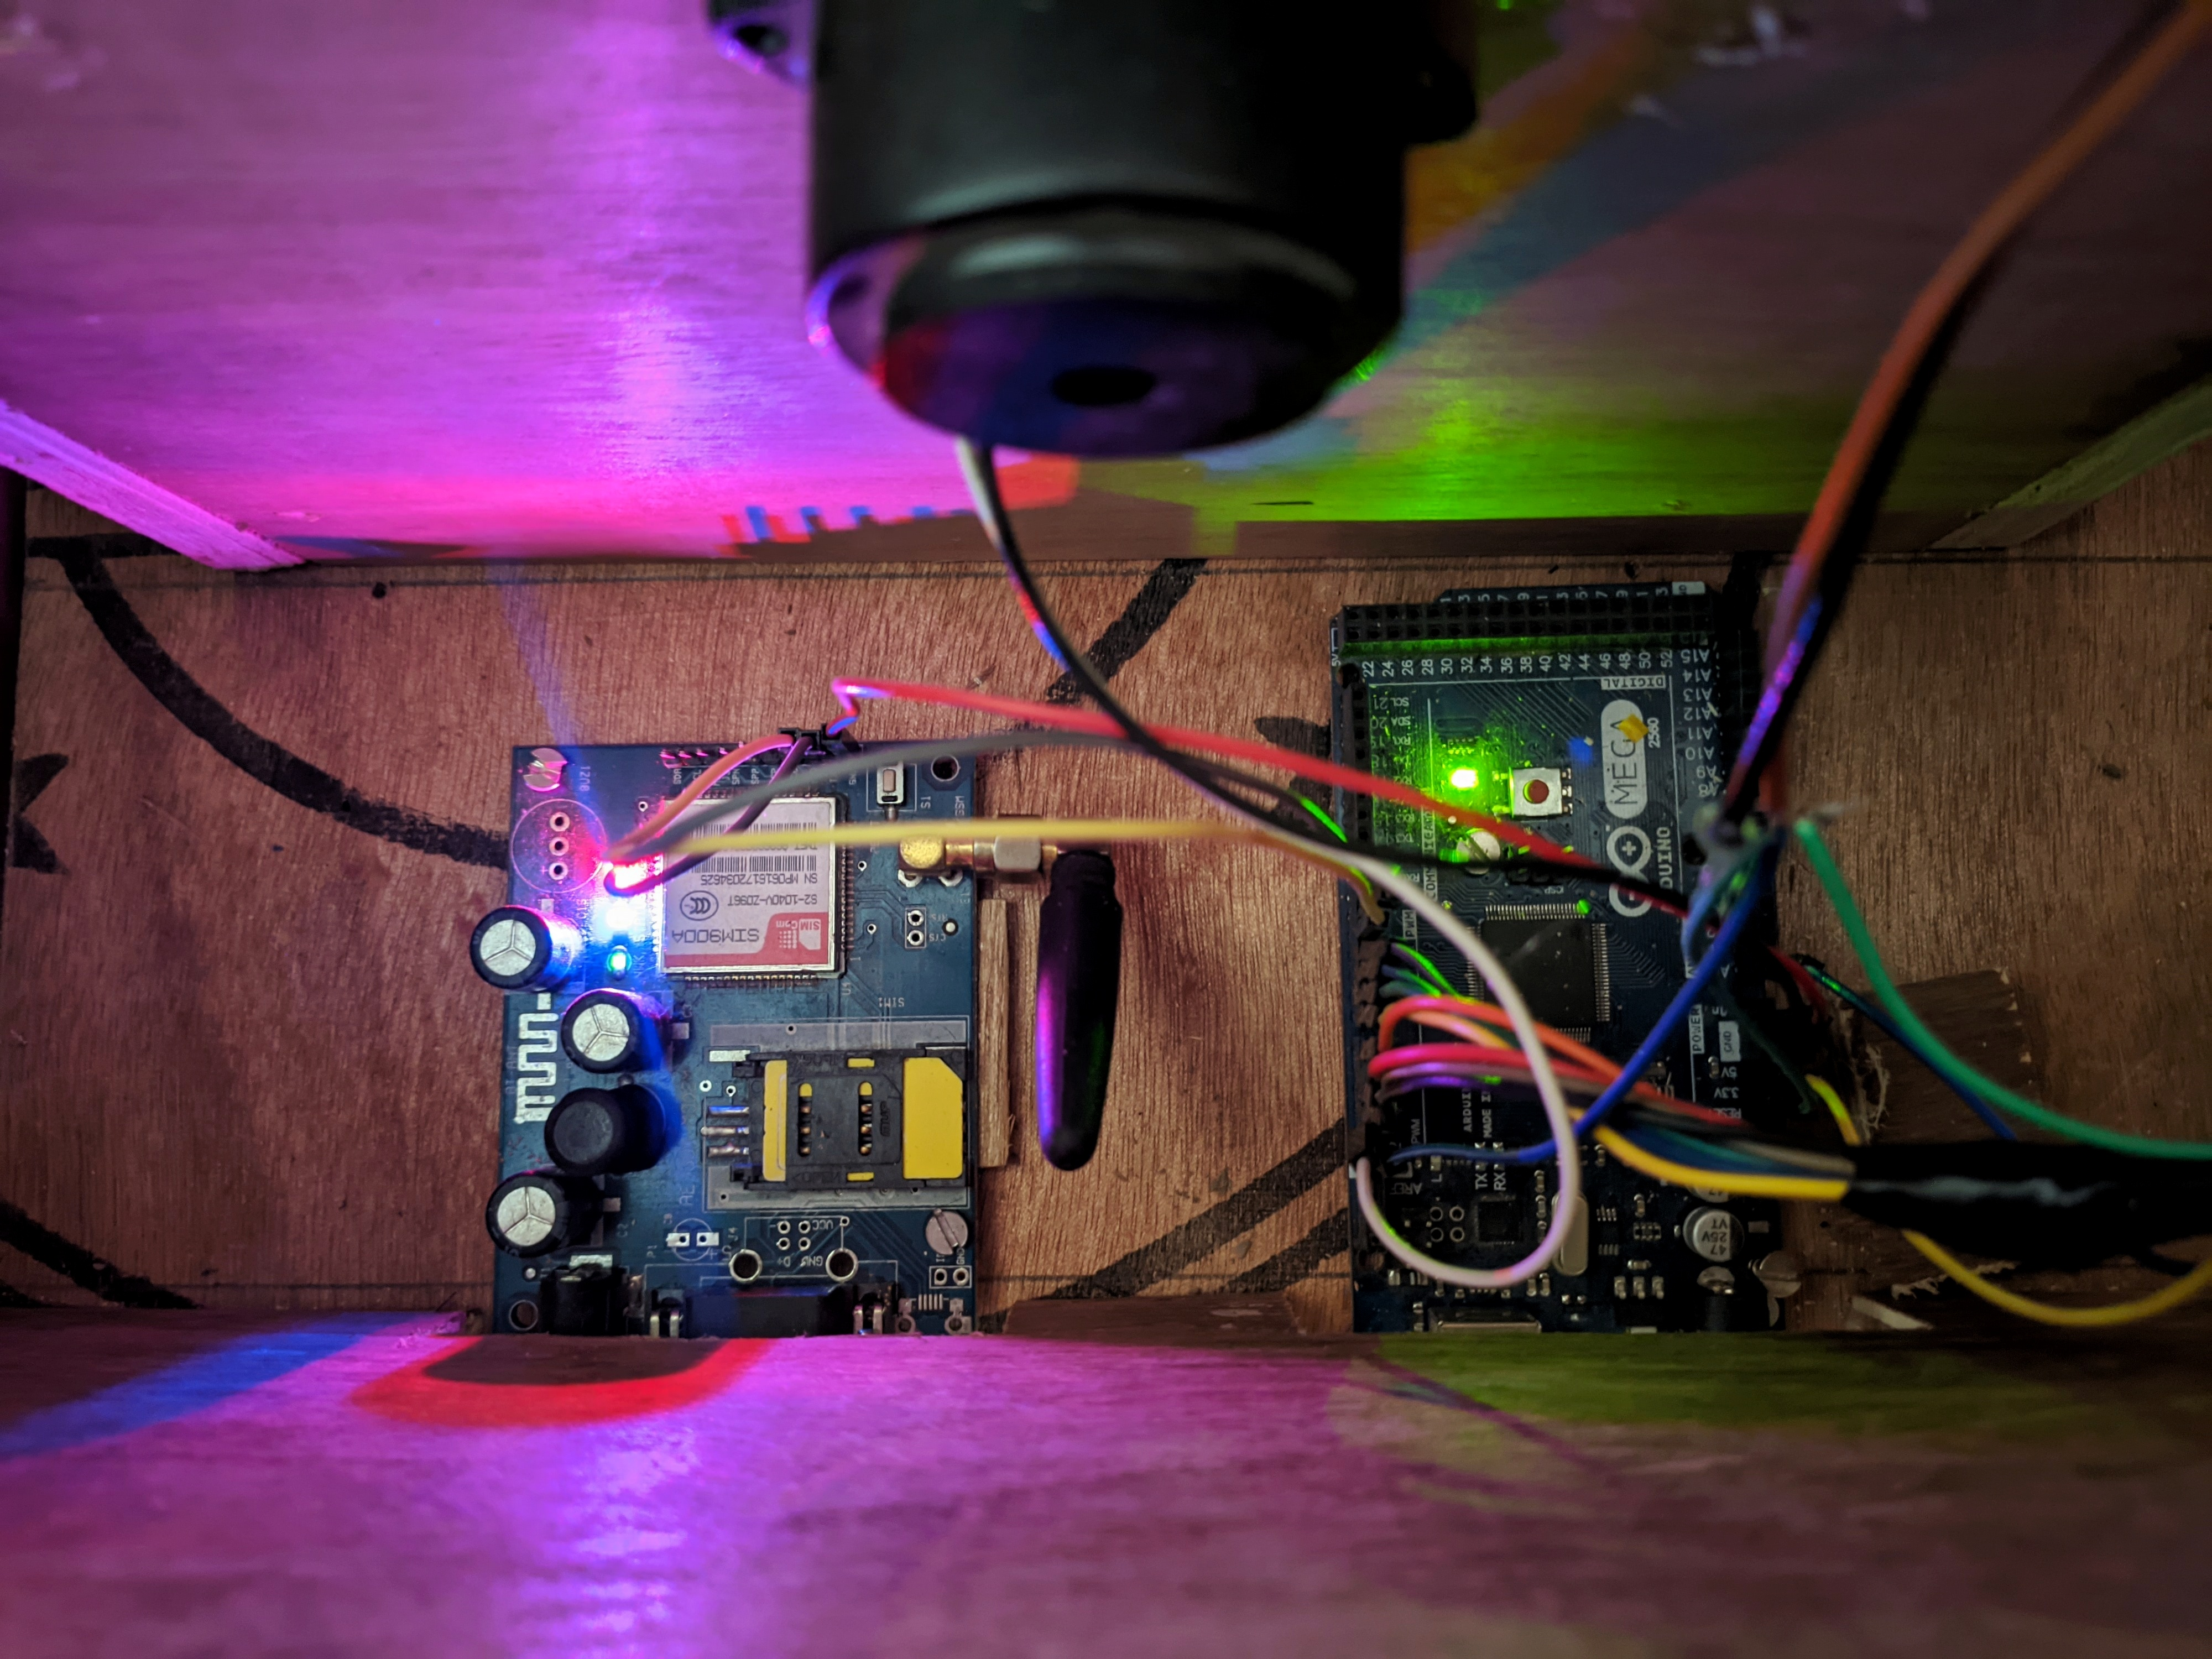
\includegraphics[height= 6cm, width=10cm]{project/images/img3}
    \caption{\textbf {back side of model }}
\end{figure}
\begin{figure}[H]
  \centering
    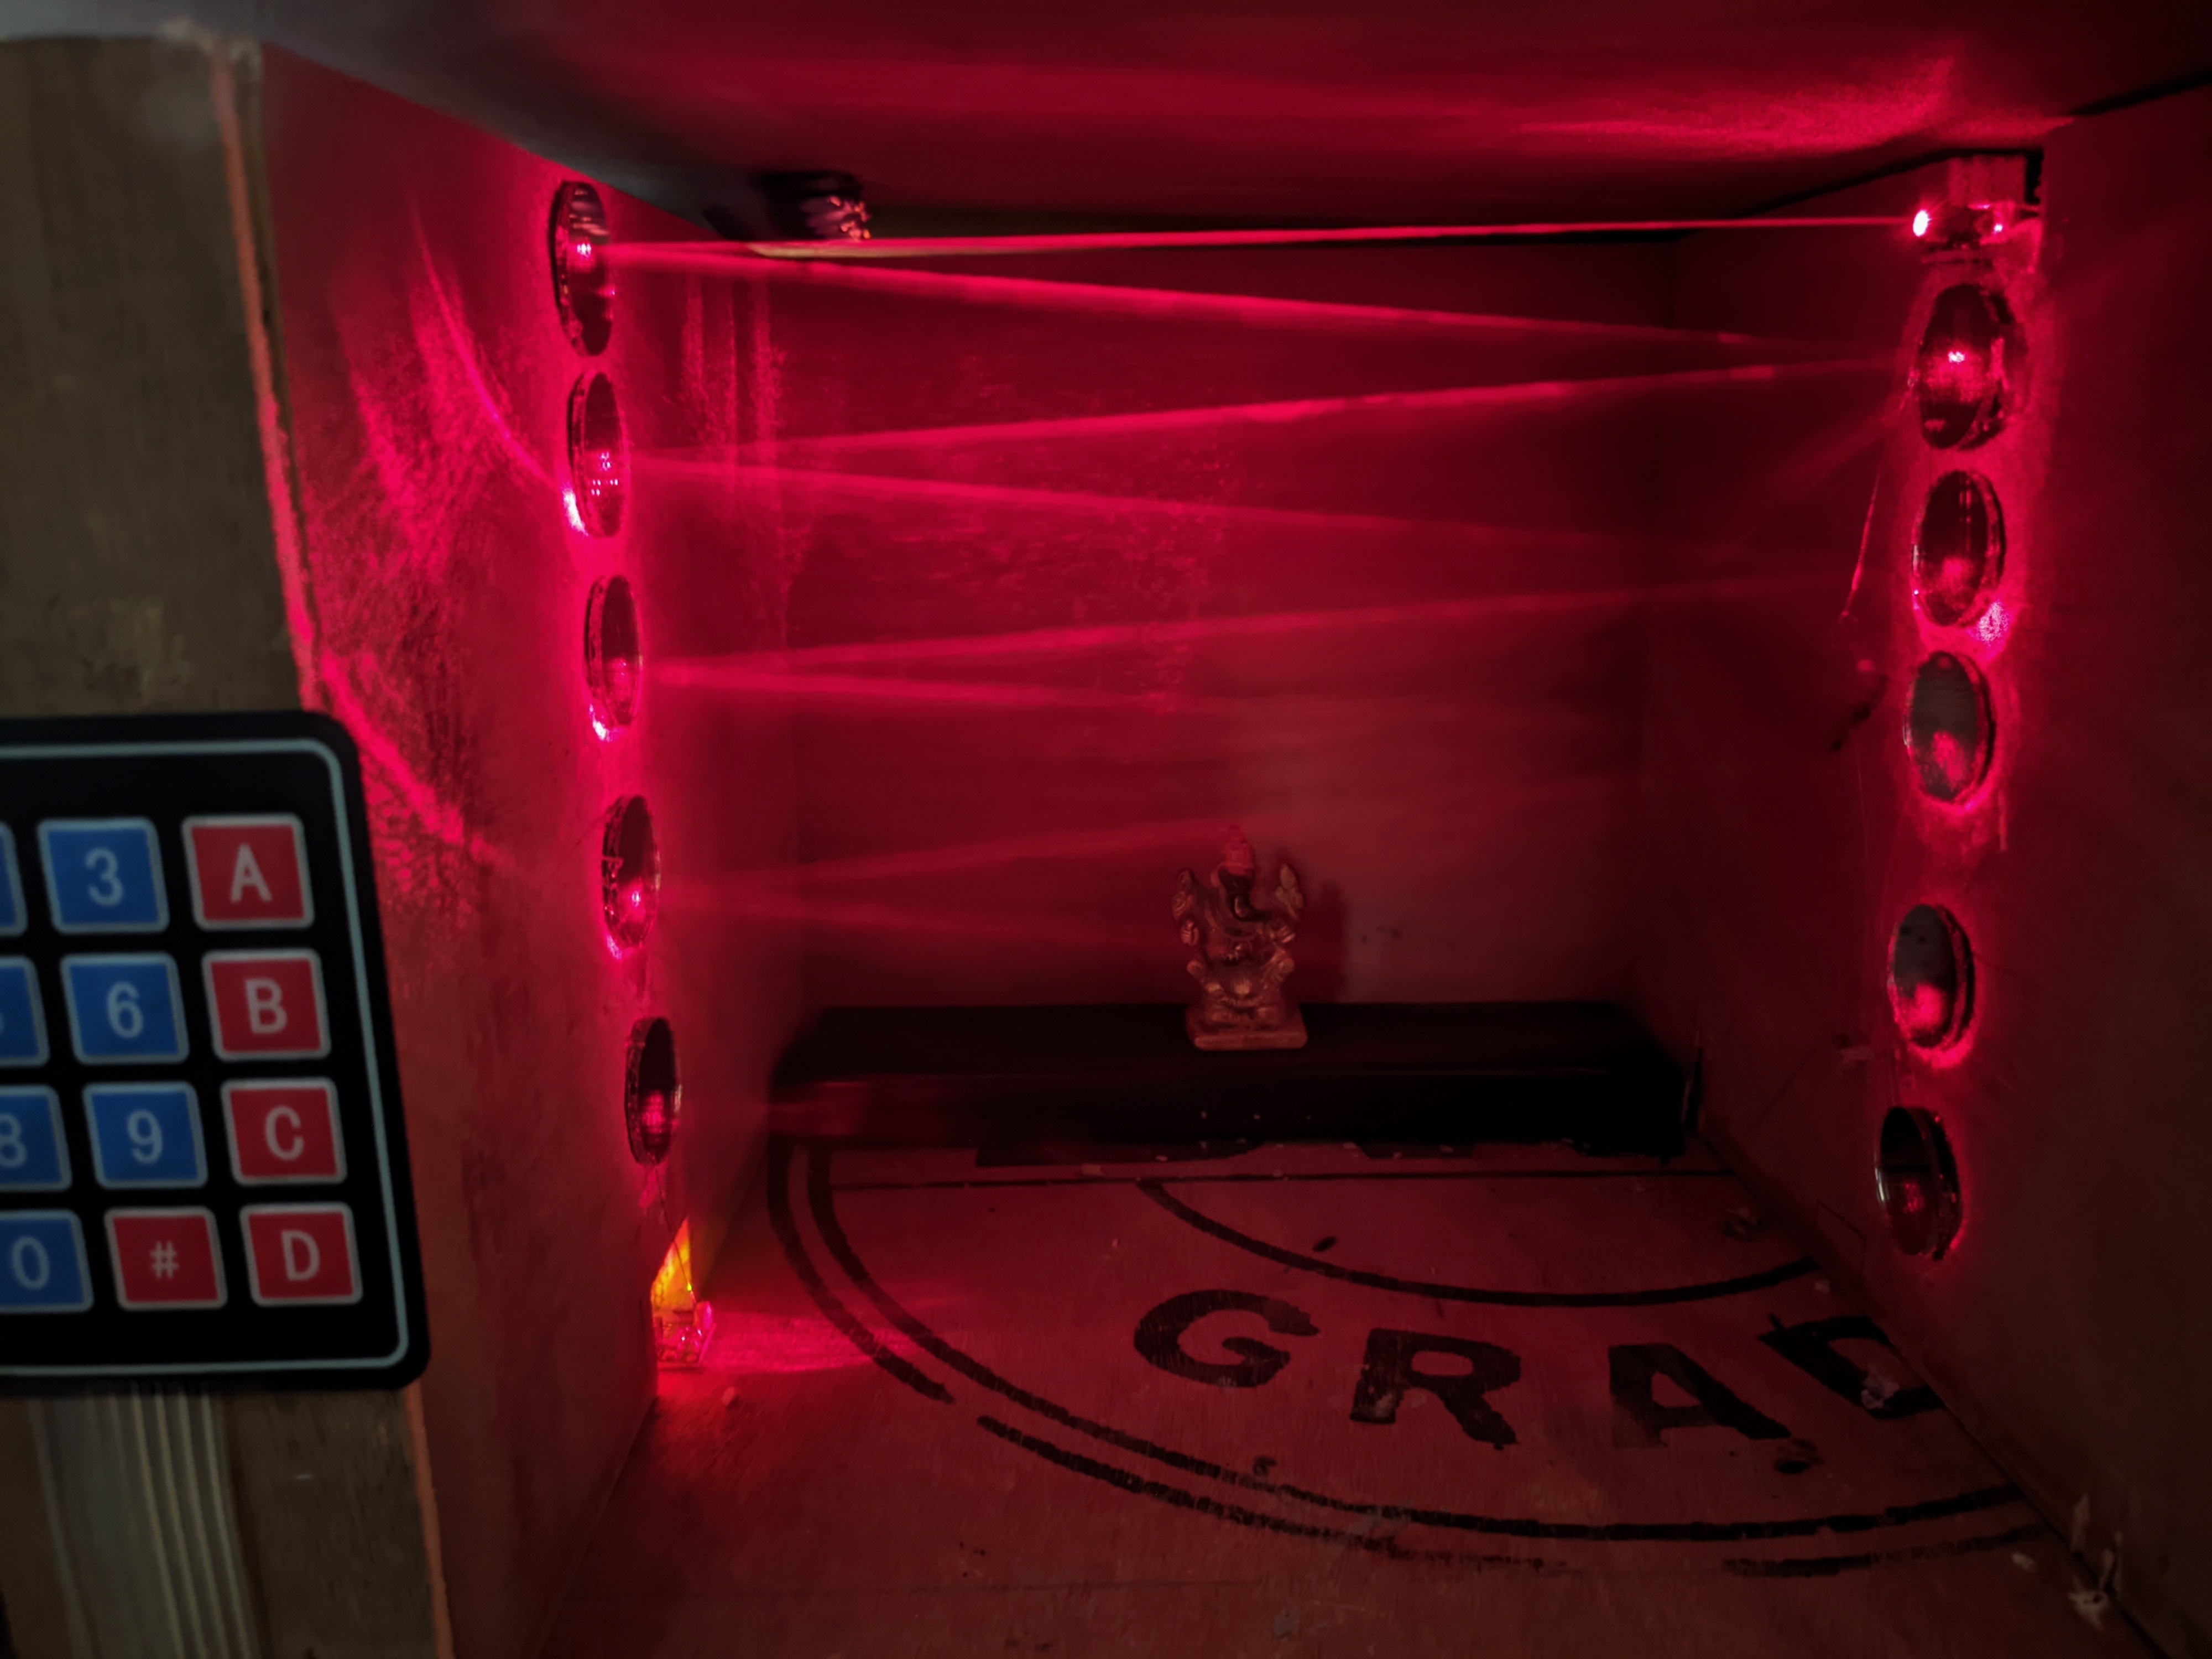
\includegraphics[height= 6cm, width=10cm]{project/images/img4}
    \caption{\textbf {establish lazer in model }}
\end{figure}

\chapter{Conclusion and Future Scope}
\section{Conclusion}


\paragraph{}Laser security system provides us the security against any crime, theft in our day to day life and so people are installing them in order to stay safe, secure and sound. Various electronic security systems can be used at home and other important working places for security and safety purposes. It is a great opportunity and source of saving man power contributing no wastage of electricity. The "Laser Security System" is an important helping system. Using this system robbery, thefts and crime can be avoided to large extend. Avoiding thieves results in the safety of our financial assets and thereby this system provides us protection against all.The Laser and LDR system is highly sensitive with a great range of working. The system senses  the  light  emitted  by  the  Laser  falling  over  the  LDR  connected  with  the  circuit. Whenever the beam of light is interrupted by any means, it triggers the alarm or siren. This highly reactive approach has low computational requirement, therefore it is well suited to surveillance, industrial application and smart environments.
\section{Future Scope}
\paragraph{}1.This security system is helpful for various security purposes.
\paragraph{}2.This type of security system easily identify the  thief or any person who try to break the system
\paragraph{}3.This type of security system can be used in various field such as bank locker , farm ,room
 % adds the Scheduling and Planning page
\addcontentsline{toc}{chapter}{References}
\begin{thebibliography}{99}
\bibitem{WRITE A SHORT-NAME WITHOUT SPACE} \emph{IEEE spectrum ( May 2009), the 555 was selected as  one of the” 25 Micro- chips that  shook the world”. }

\bibitem{WRITE A SHORT-NAME WITHOUT SPACE} \url{https://www.arduino.cc/}
\end{thebibliography} % adds the References page

\end{document}